\bookpart{流形}{Manifolds}
\label{part:manifolds}

\BookPartGuide{%
当允许的对象受到几何约束时，普通的向量运算未必仍得到允许的对象。例如，圆上两点的平均值通常不在圆上。我们需要新的方法记录位置、描述可行的变化方向，并比较沿约束空间移动的路径。

本部分以非线性空间与流形为中心，先区分对象、坐标和有限观测，再讨论距离、邻域、对称与连接等结构；随后通过映射、切向变化、约束方程和优化描述可行的计算。最后考察收敛、有限逼近以及扰动对结论的影响。

阅读时要区分连续的几何模型与带噪的有限观测：观测距离可以为重构提供信息，但误差和采样方式也会影响结果；局部坐标有用，也不意味着整个空间都能由一组坐标无歧义地覆盖。}

\chapter{非线性空间与流形}
\label{chap:differential-geometry-and-symmetry}

上一章在固定向量空间中区分了对象、坐标与线性变换。现在把可选对象限制在一个圆上：
两个圆上点的平均值通常不在圆上，沿切线走有限一步也会离开圆。怎样记录位置、选择
可行的变化方向，并比较两点之间的路程？这些问题不能只靠换一组基解决，因为限制来自
可行集合本身。即使每个小邻域都近似平直，局部记录也未必能拼成一组全局坐标。

本章以平面中的弯曲点带连接这些问题。连续带、它的中心线和带噪观测是不同对象：
带有纵横两个自由度，中心线只有一个；测量误差则描述观测怎样偏离潜在点，不自动增加
潜在空间的自由度。有限点间距离可以帮助重构坐标，对称变换说明哪些记录代表等价输入，
邻域关系则补充连通与环的信息。它们各自回答一种表示问题，不是四种互斥的空间类型。

在确定光滑流形这一连续模型以后，局部线性化给出可行速度，度量给速度规定长度，
路径积分再定义路程和距离。比较不同位置的方向还需要额外的搬运规则，由此才能讨论
局部直行与曲率。本章用已知函数和向量场描述几何与目标，但优化未知量只是流形中的点；
下一章再把整个函数或场本身作为可变对象。以下主要使用基础分析、线性代数和前文优化知识；有限距离模型与
组合拓扑模型本身不被假定为光滑流形。
本章还用两种具体对象检查“表示不等于对象”：同一比例方向可以有许多齐次坐标，
同一次三维旋转也可以有不同轴角或互为相反数的四元数记录。
前者在等价关系中建立射影坐标，并把点对应写成齐次估计；
后者在位置更新中从正交约束推导可行方向，再计算旋转与插值。
光学相机怎样产生这些观测由应用卷说明，这里建立可以复用的几何对象与运算。

\section{元素与表示}
\label{sec:geometry-nonlinear-representations}

点带上的一个潜在位置可以由$(s,u)$记录，测量得到的环境坐标则可能带误差。
这两种记录不能直接互换：前者需要先确定连续可行集合，后者还包含测量过程。
下面先界定对象，再建立局部坐标与重叠区域中的坐标转换。

\subsection{对象与空间的界定}
\label{sec:geometry-objects}

圆上两个点的和通常不在圆上，所以可行位置不能直接组成上一章的向量空间。
本章改用局部有限自由度描述可行集合。建模时要分别指定连续集合、容纳它的环境空间和有限观测：
集合限制哪些位置可行，环境坐标记录位置，观测则提供关于未知位置的信息。

上一章的空间允许我们把任意两个对象相加、按任意倍数缩放，而这里做不到，这就是需要新工具的原因。
举三个具体障碍。第一，把圆周上两个点取平均，
$\bigl((1,0)^\top+(0,1)^\top\bigr)/2=(1/2,1/2)^\top$的长度是$\sqrt2/2$而不是$1$，
平均结果掉到了圆内，对圆不再可行；对整条曲线的平均则可以。
第二，从$(1,0)^\top$沿切线方向$(0,1)^\top$走一步得到$(1,1)^\top$，
这也不在圆上；切向可行只说明一阶方向对，不说明有限步仍然可行。
第三，圆上“两个方向之间差多少”会随当前位置改变：
在$(1,0)^\top$处朝上的方向与在$(-1,0)^\top$处朝上的方向都属于切空间，
却不能直接相减比较，因为它们是两个不同平面的向量。
换一组基解决不了这些问题，因为限制来自可行集合本身的形状，而不来自记录方式。
处理办法是把“整体是平的”放宽为“每个点附近可以用有限个坐标记录”，
再另外规定怎样比较不同位置的方向和距离。这就是本章余下的任务。

图~\ref{fig:vol1-add-geometry-circle-average}把第一个障碍画出：线性组合在环境平面内仍有意义，却可能离开规定的可行集合。后面引入局部坐标，正是为了把“能在环境中计算”与“计算后仍可行”分开。
\begin{figure}[!htb]
  \centering
  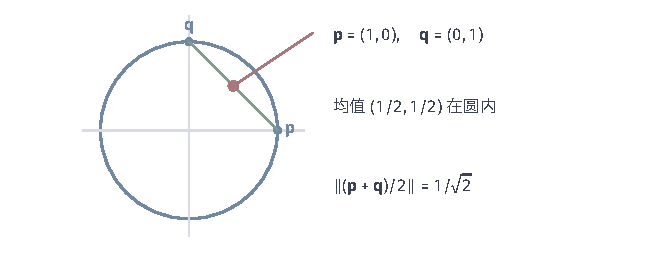
\includegraphics[width=112mm]{figures/00-shared/mathematical-preliminaries-upper/05-space-and-geometry/tikz/comprehension-additions/geometry-circle-average.pdf}
  \caption{圆周约束不对取平均封闭。蓝圆是单位圆，$\bm p=(1,0)^\top$与$\bm q=(0,1)^\top$都可行；红点是弦的中点$(\bm p+\bm q)/2$，其长度为$1/\sqrt2$，落在圆内。绿色弦位于环境平面，不是圆周上的可行路径。}
  \label{fig:vol1-add-geometry-circle-average}
\end{figure}


贯穿本章的\term{弯曲点带}取为
\begin{equation}
 \Phi(s,u)=
 \begin{bmatrix}
 (R+u)\cos(s/R)\\(R+u)\sin(s/R)
 \end{bmatrix},
 \qquad s\in I,\quad |u|<w,\quad 0<w<R,
 \label{eq:geometry-curved-strip-parameterization}
\end{equation}
其中$R>0$，$I=(s_-,s_+)$的长度小于$2\pi R$，防止绕回后重复。
$s$沿中心线定位，$u$记录横向偏移。定义
\[
 \mathcal M_{\mathrm{strip}}=\{\Phi(s,u):s\in I,\ |u|<w\},
 \qquad \mathcal C=\{\Phi(s,0):s\in I\}.
\]
前者是二维开带，后者是一维中心线，二者均不包括端点。
这里的“弯曲”首先指中心线和参数坐标线的形状。注意这是画在平面上的弯曲，
不是内在的弯曲：二维开带仍是平面的开集，采用平面欧氏长度时，每个内部点附近的
几何仍与平面完全相同。坐标线弯曲不自动意味着内在曲率非零，后面的球面例将给出
不同的局部几何——那里无论怎样选坐标，都无法把一小块摊平到平面上而不改变距离。
连续双射且逆映射也连续，称为同胚（homeomorphism）；它保留连续性关系。
开带与开矩形同胚，中心线与开区间同胚。
其参数化是否满秩将在计算局部方向时直接核对。

从这个连续模型采样时，\term{潜在点}（latent point）
$\bm p_i=\Phi(s_i,u_i)$指误差发生前的真实位置，
$\bm x_i=\bm p_i+\bm\epsilon_i$才是观测。二维开带是$\mathbb R^2$的开集，
故内部点足够小的扰动仍在带内，但不等于原潜在点；无噪声界则不保证仍在带内。
若选择的潜在对象是一维中心线，就要求$u_i=0$，把横向偏离归入观测误差。
一般扰动会将观测推出中心线，不能一面声称潜在对象一维，一面又把误差当作第二个
内在坐标。有限点云宽度很小也不足以决定这项建模选择。

图~\ref{fig:vol1-add-geometry-latent-noise}固定相似的带状外观，比较两种对象约定。左图只把中心线位置当作潜在自由度，横向偏离由观测误差解释；右图允许潜在位置本身在带内横向变化，因而多出一个内在自由度。
\begin{figure}[!htb]
  \centering
  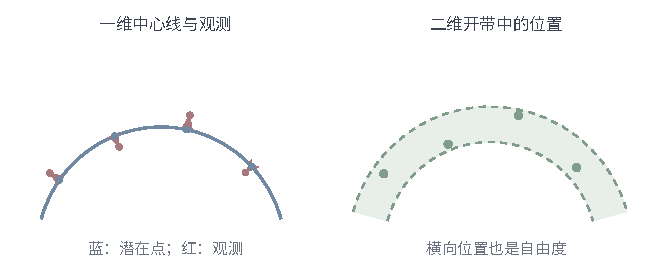
\includegraphics[width=112mm]{figures/00-shared/mathematical-preliminaries-upper/05-space-and-geometry/tikz/comprehension-additions/geometry-latent-noise.pdf}
  \caption{潜在维数取决于建模对象。左图蓝点在一维圆弧上，红点为加入四个固定径向偏移后的观测，短箭头连接对应潜在点与观测；右图绿色点是二维开带内的可行位置，虚线边界不属于开带。两图是确定性的教学示意，不以观测点的宽度估计潜在维数。}
  \label{fig:vol1-add-geometry-latent-noise}
\end{figure}



\subsection{对象的局部坐标表示}
\label{sec:geometry-manifold-coordinates}
\label{sec:geometry-local-coordinate-representation}

\label{sec:geometry-local-charts}

在圆的一小段上，一个角度便能定位一个点；绕完整圆却必然遇到角度断点或重复表示。
\term{流形}（manifold）把这两件事分开：它要求每个点附近像某个欧氏开集，
并不要求整个对象是一张欧氏坐标表。本章先讨论欧氏空间中的光滑嵌入流形；
光滑指各阶导数连续，微分同胚指映射及其逆都光滑\scite{math-lee2013smooth}。

\begin{definition}[光滑嵌入流形]
\label{def:geometry-embedded-manifold}
设$0\leq d\leq D$。集合$\mathcal M\subseteq\mathbb R^D$称为$d$维光滑嵌入流形，
若每个$\bm p\in\mathcal M$都有包含它的环境开集$O$和欧氏开集之间的微分同胚
$\Psi:O\to\Psi(O)\subseteq\mathbb R^D$，满足
\[
 \Psi(\mathcal M\cap O)
 =\Psi(O)\cap(\mathbb R^d\times\{\bm0_{D-d}\}).
\]
\end{definition}
这个条件用已经学过的欧氏光滑映射把对象局部拉直，因而没有用“流形上的光滑逆”
循环定义流形。前$d$个坐标描述局部自由度，$D$只是容纳对象的环境维数。

令$U=\{\bm z:(\bm z,\bm0_{D-d})\in\Psi(O)\}$，则
$\varphi(\bm z)=\Psi^{-1}(\bm z,\bm0_{D-d})$从开集$U\subseteq\mathbb R^d$
参数化$\mathcal M\cap O$，且Jacobian满列秩。一般局部参数化还须在其像上具有
连续逆；仅仅满秩并不能排除全局绕回或自交。参数化的方向是“坐标到点”，
读取一个点的位置则要使用反向映射。


参数化的逆$\chi=\varphi^{-1}:\mathcal M\cap O\to U$称为
\term{坐标图}（chart）。覆盖整个流形的一组坐标图称为图册（atlas）；
“局部像$\mathbb R^d$”指有这种局部记录方式，不是说流形在环境中必须平直。

\subsection{坐标的转换}
\label{sec:geometry-coordinate-conversions}

同一点可能由两张图记录。要让这两份记录兼容，需要明确坐标之间的转换。
\begin{definition}[坐标过渡]
\label{def:geometry-chart-transition}
两张图的覆盖区域相交时，$\chi_2\circ\chi_1^{-1}$把第一组坐标换成第二组坐标，
称为\term{坐标过渡}（coordinate transition），定义在交集的第一组坐标像上。
\end{definition}
坐标过渡及其逆都光滑，因此在重叠区域中换图不改变光滑性。

单位圆的参数化$\varphi(\theta)=(\cos\theta,\sin\theta)^\top$限制到
$(-\pi,\pi)$时漏掉$(-1,0)^\top$，限制到$(0,2\pi)$时漏掉$(1,0)^\top$。
两张图合起来覆盖圆，交叠处的过渡是$\theta$或$\theta+2\pi$。
断点移动的是坐标，不是圆被切断了。
完整圆是紧集，它在连续映射下的像仍紧；非空的一维欧氏开集却不紧，
所以圆不可能与这种开集同胚，也不能靠一张无重复的实数坐标图覆盖。
它局部一维，却至少需要二维环境才能
无自交地全局嵌入；局部维数、环境维数与最小全局嵌入维数由不同条件决定。图~\ref{fig:geometry-circle-chart-transition}给出同一圆上两个点在两张图中的记录。

\begin{figure}[htbp]
  \centering
  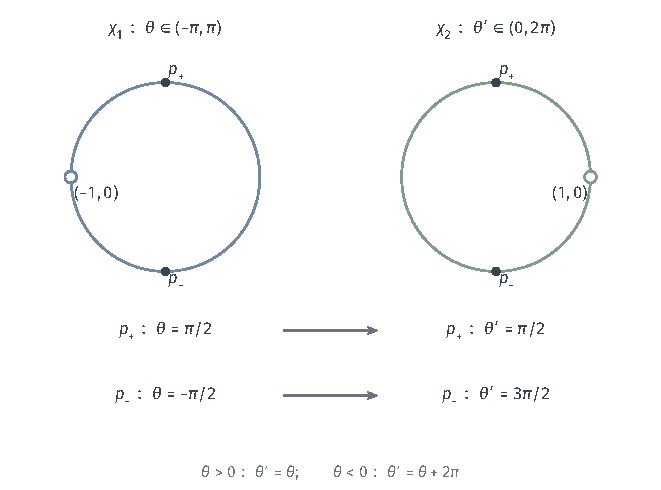
\includegraphics[width=112.0mm]{figures/00-shared/mathematical-preliminaries-upper/05-space-and-geometry/tikz/geometry-circle-chart-transition/figure.pdf}
  \caption{单位圆的两张坐标图。空心点分别是各图漏掉的$(-1,0)^\top$与$(1,0)^\top$，两图合起来覆盖完整圆。两图中的$p_+$相互对应，$p_-$也相互对应；每对标记记录同一个几何点。上半圆过渡保持角度，下半圆过渡加$2\pi$。图下方列出两个交叠分支的转换，不把坐标断点理解为圆被切断。}
  \label{fig:geometry-circle-chart-transition}
\end{figure}




同一个点在两张图中的坐标不同，过渡映射必须把旧记录送到新记录。
三张图共同覆盖时，$\chi_3\circ\chi_1^{-1}
=(\chi_3\circ\chi_2^{-1})\circ(\chi_2\circ\chi_1^{-1})$，
等式只在各步都有定义的重叠区域使用。与线性换基相同，中间记录消去；
不同之处在于过渡通常非线性且只在局部有效。

\section{关系与结构}
\label{sec:geometry-relations}

两条圆弧在小邻域中都可以用一个坐标记录，却可能属于不同的连通分支；
同一圆上的两点也有不同切线。局部坐标之外，还需建立邻域、切向与距离关系，
分别描述连续连接、可行速度与路线代价。若任务要忽略旋转或重编号，再以等价关系规定这种忽略。
同样的等价语言还处理比例未知的记录：先把非零倍数归为一个点，再选择局部坐标，
就能解释无穷远位置和点线对应。后者用线性方程估计，但被估计的对象是射影变换，
不能把齐次参数向量的普通长度当作对象本身的几何大小。

\subsection{对象的邻域关系}
\label{sec:geometry-neighborhood-relations}
\label{sec:geometry-local-relations-topology}

\label{sec:geometry-neighborhood-topology}

在嵌入模型中，$\mathcal M\cap O$（$O$为环境开集）给出相对开集。
包含一个含有该点的相对开集的集合，称为该点的邻域。开集的任意并、有限交仍开，
它们决定连续映射、连通与局部记录所需的关系。
两条互不相交的开圆弧和一条完整圆，每个点附近都像一维开区间，
整体却分别有两个连通分支和一个不可在圆内缩到点的环。
\term{拓扑}（topology）在这里研究连续连接与孔洞等结构，
不要求保持长度和角度。把开点带连续拉直可以保留连接关系，
把两端粘合却改变了对象。局部自由度不能回答这种整体问题。

为什么这类问题不能用坐标或距离直接回答？两组点可以有完全相同的个数、
两两距离也按某种重排相同，一个围成空心环、另一个内部填满，区别只在
“中间有没有面”。因此要把形状变可计算，光给出顶点和边还不够，
还必须补充一条组合信息：哪些点围成的形状被当作已填充。
下面先用最简单的单纯形把“点—边—面”记录下来，再让边界运算自动区分
“只是一圈边”和“这圈边已被面填上”。

有限欧氏点集继承的拓扑是离散的：每个点自成一个开集，样本再多也推不出“哪些点相连”。
要从样本推测连续形状，必须另行规定哪些点集算作被填充的单元，也就是补充组合信息；
否则只知道有一批点，不知道它们之间有没有面。一种做法是记录一族顶点子集：
单点是一条记录，多点子集表示这些点围成的形状被填充。为使含$k+1$个顶点的单元
确实张成$k$维形状，要求以一个顶点$\bm v_0$为基点时，差向量
$\bm v_1-\bm v_0,\ldots,\bm v_k-\bm v_0$线性无关；
这称为顶点的仿射独立（affine independence），三个顶点时就是不共线。
$k$维\term{单纯形}（simplex）在几何上是这些顶点的凸包，在组合表示中只记录顶点集合。
点、线段、填充三角形分别是零、一、二维单纯形。
仿射独立保证几何维数；组合形式则用于指定哪些高阶面存在。

\begin{definition}[抽象单纯复形]
\label{def:geometry-simplicial-complex}
有限顶点集上的\term{抽象单纯复形}（abstract simplicial complex）
$\mathcal K$是一族非空顶点子集，满足向下封闭：
\begin{equation}
 \sigma\in\mathcal K,\quad\varnothing\neq\tau\subseteq\sigma
 \quad\Longrightarrow\quad\tau\in\mathcal K.
 \label{eq:geometry-simplicial-complex-closure}
\end{equation}
含$k+1$个顶点的元素称为$k$维单纯形。
\end{definition}
加入三角面必须连同它的三条边和三个顶点一起加入，反之不成立。
这使复形能够区分“围出一圈”和“这一圈已由一个面填充”。

这些顶点子集如何成为可以讨论连续路径的空间？以三个顶点为例，
只取三条边就把三条线段沿同名端点粘成一圈；再加入三角面，就把内部也填上。
对有限顶点集$\{1,\ldots,m\}$，可以把第$i$个顶点放在$\mathbb R^m$的单位向量$\bm e_i$处，
将每个$\sigma\in\mathcal K$实现为相应单位向量的凸包。所有这些面的并集为
\[
 |\mathcal K|=
 \left\{\bm a\in\mathbb R^m:
 a_i\geq0,\ \sum_i a_i=1,\ \{i:a_i>0\}\in\mathcal K\right\},
\]
配上从$\mathbb R^m$继承的拓扑，称为复形的\term{几何实现}（geometric realization）。
公共面由相同顶点自动识别，向下封闭保证这些面也在复形中。
这里的单位向量只是实现组合粘合关系的坐标，不要求等于原观测点的位置；
后文谈复形的同伦类型时，比较的正是这个拓扑空间。


为计算未被填充的环，需要把端点抵消与高阶填充分别记录。
选定顶点次序后，以$[v_0,\ldots,v_k]$表示有向单纯形，交换两顶点使符号反转。
有向$k$维单纯形的实系数线性组合称为$k$维链，
组成向量空间$C_k(\mathcal K;\mathbb R)$。边界算子读取每个面的有向边缘：
\begin{equation}
 \partial_k[v_0,\ldots,v_k]
 =\sum_{i=0}^k(-1)^i[v_0,\ldots,\widehat{v_i},\ldots,v_k],
 \qquad k\geq1,
 \label{eq:geometry-simplicial-boundary}
\end{equation}
尖帽表示删去该顶点，算子线性延伸到全部链。
本章采用非约化同调，约定$C_{-1}=\{0\}$、$\partial_0=0$。
例如$\partial_1[1,2]=[2]-[1]$，端点的正负表示方向。

\begin{lemma}[边界的边界为零]
\label{lem:geometry-boundary-squared-zero}
上述算子满足
\begin{equation}
 \partial_{k-1}\partial_k=0,\qquad k\geq1.
 \label{eq:geometry-boundary-squared-zero}
\end{equation}
\end{lemma}
\begin{proof}
$k=1$时由$\partial_0=0$成立。对$k\geq2$，固定$i<j$，
两次删除$v_i,v_j$后得到相同的$(k-2)$维面。
先删$i$再删原来的$j$，系数为$(-1)^i(-1)^{j-1}$；
先删$j$再删$i$，系数为$(-1)^j(-1)^i$，两者相反。
所有项都按这样的顶点对成对抵消，因此结论对基单纯形成立；
由线性性，对全部链成立。
\end{proof}

边界必定闭合，但闭合的圈未必由复形中的某个面填充。
这正好可以用上一章的核、像与商空间表达。
\begin{definition}[闭链、边界与同调空间]
\label{def:geometry-homology-space}
满足$\partial_kc=0$的链称为\term{闭链}（cycle），
能写成$c=\partial_{k+1}b$的链称为\term{边界}（boundary）。
由$\partial_k\partial_{k+1}=0$，有
$\operatorname{im}\partial_{k+1}\subseteq\ker\partial_k$。
实系数\term{同调空间}（homology space）及其维数定义为
\[
 H_k(\mathcal K;\mathbb R)=\ker\partial_k/\operatorname{im}\partial_{k+1},
 \qquad \beta_k=\dim H_k(\mathcal K;\mathbb R).
\]
$\beta_k$称为第$k$个\term{Betti数}（Betti number）。
\end{definition}
商空间沿用\BookDefinitionRef{def:linear-algebra-quotient-space}{定义~\ref{def:linear-algebra-quotient-space}}：
两个闭链相差一个边界时被视为同类。因而$H_k$保留的不是全部闭链，
而是无法用已有高阶填充消去的部分；$\beta_0$计算连通分支，
$\beta_1$计算实系数意义下独立的一维环。

取
$\mathcal K_{\mathrm{loop}}
=\{\{1\},\{2\},\{3\},\{1,2\},\{2,3\},\{1,3\}\}$。
链$c=[1,2]+[2,3]-[1,3]$的端点逐一抵消，故$\partial_1c=0$。
$\partial_1$的秩为$2$，一维闭链空间维数为$3-2=1$，
而没有二维面，故$\beta_1=1$、$\beta_0=3-2=1$。
加入$[1,2,3]$后，$c=\partial_2[1,2,3]$成为边界，$\beta_1$降为$0$；
$\partial_1$不变，所以$\beta_0$仍为$1$。
图~\ref{fig:geometry-cycle-filled-simplex}只改变面集合，顶点与边保持相同。
\begin{figure}[htbp]
  \centering
  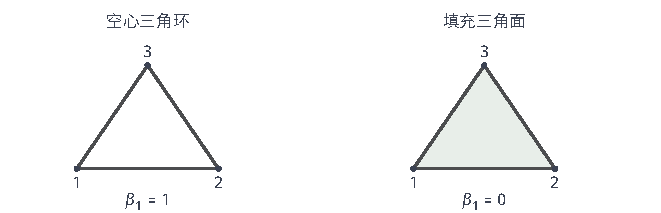
\includegraphics[width=112.0mm]{figures/00-shared/mathematical-preliminaries-upper/05-space-and-geometry/tikz/geometry-cycle-filled-simplex/figure.pdf}
  \caption{一圈边是否已填充，取决于高阶面而非边图。左侧闭链
 $c=[1,2]+[2,3]-[1,3]$不是边界；右侧加入$[1,2,3]$后有
 $c=\partial_2[1,2,3]$。两者$\beta_0=1$，$\beta_1$分别为$1$与$0$。
 图为组合教学示例，不代表某个观测点云的真实拓扑。}
 \label{fig:geometry-cycle-filled-simplex}
\end{figure}


若$N_k$是$k$维单纯形数，Euler示性数
$\chi=\sum_k(-1)^kN_k$是更粗的摘要：空心三角形为$3-3=0$，
填充三角形为$3-3+1=1$。由秩--零度关系
$N_k=\beta_k+\operatorname{rank}\partial_k+\operatorname{rank}\partial_{k+1}$，
交替求和后中间秩抵消，也得到$\chi=\sum_k(-1)^k\beta_k$。
不同Betti数组甚至不同拓扑都可能有同一个$\chi$，一个标量不足以代替分别分析。

\subsection{对象的位置与方向关系}
\label{sec:geometry-position-direction-relations}
\label{sec:geometry-manifold-local-linearization}
\label{sec:geometry-analytic-local-linearization}

从$\bm p=\varphi(\bm z)$出发，坐标变化$\bm v$经Jacobian
$\bm J_\varphi(\bm z)$映为环境空间中的瞬时速度。
\term{切空间}（tangent space）收集所有这样的可行速度；
它描述一阶方向，并不是可行集合本身的一小块。

为什么要另立这个概念？因为在曲面上做优化时，“往哪个方向走”必须先有一个明确答案，
而直接沿环境坐标的某个方向平移会离开曲面。球面上取$\bm p=(1,0,0)^\top$，
沿$\bm e_z$方向移动立刻离开球面；沿$(0,1,0)^\top$移动则只在零步长时留在球面上。
切空间把“零步长的可行方向”单独收集起来，使一阶问题可以用上一章的线性代数处理，
而把有限步可行性交给后面的位置更新。
以二维单位圆为例，$\bm p=(1,0)^\top$处的切空间是
$\operatorname{span}\{(0,1)^\top\}$，记录的是以零速度为原点的竖直方向向量。
把这些向量的起点画在$\bm p$处，才得到仿射切线
$\bm p+\operatorname{span}\{(0,1)^\top\}=\{(1,t)^\top:t\in\mathbb R\}$。
这条仿射直线与圆只在$\bm p$处相交；线性切空间本身不是这条位置直线。
因此“方向集合”和“可行位置集合”必须分开记录。

\begin{definition}[嵌入流形的切空间]
\label{def:geometry-tangent-space}
设$\varphi:U\subseteq\mathbb R^d\to\mathcal M\subseteq\mathbb R^D$
是局部参数化，$\bm p=\varphi(\bm z)$。定义
\begin{equation}
 T_{\bm p}\mathcal M
 =\{\bm J_\varphi(\bm z)\bm v:\bm v\in\mathbb R^d\}.
 \label{eq:geometry-tangent-space-chart}
\end{equation}
\end{definition}
Jacobian列满秩保证这是$d$维向量空间，其原点是零速度。
画在$\bm p$旁边的仿射切平面则是$\bm p+T_{\bm p}\mathcal M$；
点的位置与速度向量的零点不能混为一谈。

\begin{lemma}[曲线速度与坐标刻画相容]
\label{lem:geometry-tangent-curves}
$T_{\bm p}\mathcal M$恰是全部光滑曲线
$\gamma:(-\epsilon,\epsilon)\to\mathcal M$、$\gamma(0)=\bm p$
的速度$\gamma'(0)$组成的集合，并且与局部坐标选择无关。
\end{lemma}
\begin{proof}
在足够小的参数区间内，曲线落入当前坐标图，写成
$\gamma(t)=\varphi(\bm z(t))$。链式法则给出
$\gamma'(0)=\bm J_\varphi(\bm z)\bm z'(0)$，故每个曲线速度都属于所定义的空间。
反过来，任意$\bm v\in\mathbb R^d$给出曲线
$t\mapsto\varphi(\bm z+t\bm v)$；因为$U$开，足够小的$t$仍在定义域内，
其初速度为$\bm J_\varphi(\bm z)\bm v$。

若另一参数化满足$\widetilde\varphi=\varphi\circ\psi$，
坐标过渡$\psi$的Jacobian可逆，且
$\bm J_{\widetilde\varphi}=\bm J_\varphi\bm J_\psi$。
右乘可逆矩阵不改变值域，两张图因而给出同一切空间。
\end{proof}

在点带中直接求导，可核对两个自由度：
\begin{align}
 \frac{\partial\Phi}{\partial s}
 &=\left(1+\frac uR\right)
   \begin{bmatrix}-\sin(s/R)\\\cos(s/R)\end{bmatrix},
 \label{eq:geometry-strip-s-tangent}\\
 \frac{\partial\Phi}{\partial u}
 &=\begin{bmatrix}\cos(s/R)\\\sin(s/R)\end{bmatrix}.
 \label{eq:geometry-strip-u-tangent}
\end{align}
因$|u|<w<R$，第一列不为零，两列正交且线性无关；
开带的切空间是整个$\mathbb R^2$。中心线则只允许$u=0$，
\[
 T_{\Phi(s,0)}\mathcal C
 =\operatorname{span}\{(-\sin(s/R),\cos(s/R))^\top\}.
\]
径向方向对开带可行，对中心线不可行。中心线的切线随位置转动，
没有一条固定线性子空间等于各处的切空间。

图~\ref{fig:geometry-strip-tangent-coordinates}上半部把切向速度画在点旁，
下半部比较同一坐标增量对应的实际弧长。方向数目决定局部维数，
坐标增量怎样换算为长度则留待度量处理。
\begin{figure}[!htb]
  \centering
  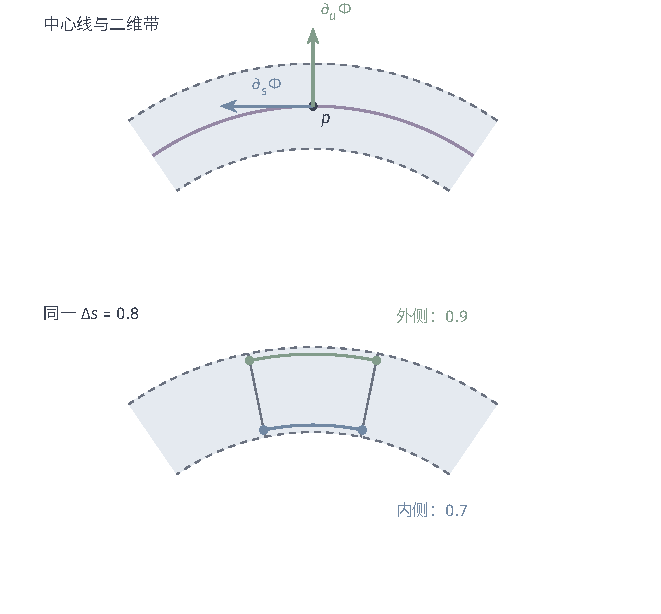
\includegraphics[width=112.0mm]{figures/00-shared/mathematical-preliminaries-upper/05-space-and-geometry/tikz/geometry-strip-tangent-coordinates/figure.pdf}
  \caption{开带与中心线的局部方向不同。取$R=2$、$w=0.3$。
 上图的两个参数方向属于二维开带，仅以中心线为对象时，径向方向不属于其切空间；
 箭头平移到$\bm p$只是画法。下图取$u=-0.25,0.25$，同一$\Delta s=0.8$
 对应圆弧长度$0.7,0.9$。灰虚线为不纳入开带的边界，两图等比例绘制，均为解析教学示例。}
 \label{fig:geometry-strip-tangent-coordinates}
\end{figure}


若流形由约束$F(\bm x)=\bm0$给出，其中
$F:\mathbb R^D\to\mathbb R^{D-d}$在$\bm p$附近光滑且
$\bm J_F(\bm p)$行满秩，就能选出$D-d$列组成可逆方阵。
重排坐标后，\BookTheoremRef{thm:analysis-implicit-function}{定理~\ref{thm:analysis-implicit-function}}把这$D-d$个变量
解为其余$d$个变量的光滑函数，后者便给出局部参数化。
对约束内曲线求导得$\bm J_F(\bm p)\gamma'(0)=\bm0$；
所以切空间包含于该矩阵的核。参数化给出$d$维切空间，
秩--零度关系又说明核为$d$维，故$T_{\bm p}\mathcal M=\ker\bm J_F(\bm p)$。
满秩条件不能省略：$F(x,y)=x^2+y^2$在原点导数为零，
核是整个平面，但零水平集只有一个点，真实可行速度只有零向量。

图~\ref{fig:vol1-add-geometry-constraint-rank}把满秩条件与退化情形并列。退化约束的导数没有排除任何方向，但约束集合本身没有非零可行速度；因此不能只求导后就把矩阵的核当成真实切空间。
\begin{figure}[!htb]
  \centering
  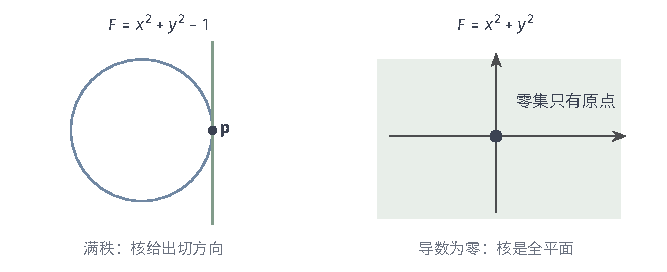
\includegraphics[width=112mm]{figures/00-shared/mathematical-preliminaries-upper/05-space-and-geometry/tikz/comprehension-additions/geometry-constraint-rank.pdf}
  \caption{约束导数的核需要满秩条件。左图$F(x,y)=x^2+y^2-1$在$\bm p=(1,0)$处导数为$(2,0)$，绿色核方向是圆的切方向，画在$\bm p$旁作为仿射切线。右图$F(x,y)=x^2+y^2$的零集只有原点，而该点导数为零，绿色底色表示其核是整个平面。}
  \label{fig:vol1-add-geometry-constraint-rank}
\end{figure}



\subsection{对象的距离关系}
\label{sec:geometry-metric-length-distance}
\label{sec:geometry-metric-path-geodesic}
\label{sec:geometry-same-point-metric}

\label{sec:geometry-riemannian-metric}
\label{sec:geometry-path-speed-length}
\label{sec:geometry-endpoint-distance}
\label{sec:geometry-continuous-geodesic-distance}

切空间说明方向可不可行，却没有规定一单位坐标变化有多长。
点带外侧与内侧相同的$\mathrm ds$对应不同弧长，因而内积必须按位置指定。
\term{Riemann度量}（Riemannian metric）为每个切空间提供这种长度与夹角规则。

在局部参数化$\varphi$中，把坐标记为$(z^1,\ldots,z^d)$；
上标在这里是坐标编号。相应坐标切基为
$\partial_i=\partial\varphi/\partial z^i$。

\begin{definition}[Riemann度量]
\label{def:geometry-riemannian-metric}
光滑流形$\mathcal M$上的Riemann度量$g$为每个$\bm p$指定内积
$g_{\bm p}:T_{\bm p}\mathcal M\times T_{\bm p}\mathcal M\to\mathbb R$，
且在任一光滑坐标切基$\partial_i$中，矩阵
$\bm G(\bm z)=[g_{i,j}(\bm z)]$、$g_{i,j}=g(\partial_i,\partial_j)$
的条目光滑。每个$\bm G$都对称正定。
\end{definition}
对同点切向量$\bm v,\bm w$，长度为
$\lVert\bm v\rVert_g=\sqrt{g_{\bm p}(\bm v,\bm v)}$；
非零时夹角满足
$\cos\vartheta=g_{\bm p}(\bm v,\bm w)/
(\lVert\bm v\rVert_g\lVert\bm w\rVert_g)$。
若它们的坐标分量为$\bm a,\bm b$，内积是$\bm a^\top\bm G\bm b$。
$\bm G$既不是样本协方差，也不必是全空间共享的常矩阵。

可以把$\bm G$想成速度表的换算器。坐标告诉我们参数每秒变化多少，
但“参数变化$1$”本身不是物理快慢：在点带外弧上，
同样的$\dot s=1$对应的实际速度比内弧大。要把坐标读数换算成真实速率、
并判断两个速度是否垂直，就需要在每个位置放一个换算矩阵；
这正是度量随位置指定内积的原因。

嵌入流形可以限制环境欧氏内积，得到诱导度量：
\begin{equation}
 \bm G(\bm z)=\bm J_\varphi(\bm z)^\top\bm J_\varphi(\bm z).
 \label{eq:geometry-induced-metric}
\end{equation}
对非零$\bm a$，满列秩保证
$\bm a^\top\bm G\bm a=\lVert\bm J_\varphi\bm a\rVert_2^2>0$。
若Jacobian退化，只会得到半正定形式；这不符合当前坐标中的Riemann度量条件。
也可以另选光滑正定内积，但这样会改变几何，而不只是改写坐标。

若旧坐标$\bm z=\psi(\bm v)$，记可逆Jacobian为$\bm A=\bm J_\psi$，
同一几何向量的旧分量等于$\bm A$乘新分量，所以
\begin{equation}
 \widetilde{\bm G}(\bm v)=
 \bm A^\top\bm G(\psi(\bm v))\bm A.
 \label{eq:geometry-metric-coordinate-transform}
\end{equation}
因此$\bm a^\top\widetilde{\bm G}\bm b
=(\bm A\bm a)^\top\bm G(\bm A\bm b)$。
改变分量而不改变度量会改变所计算的长度；按此式一起变换则仍描述同一内积。

沿中心线$u=0$可以具体看出坐标、切向量与度量的分工。
角度$\theta=s/R$记录位置；运动对时间求导后，$\dot\theta$对应的环境速度长度为
$R|\dot\theta|$。改用弧长坐标$s$，同一速度的分量变成$\dot s=R\dot\theta$，
长度写成$|\dot s|$。坐标给位置记数，切向量给允许的一阶变化，度量把变化读成长度；
这三项合起来仍没有规定有限一步怎样到达另一个可行点，位置更新还要构造流形内的路径。

点带的两个参数方向已在式~\eqref{eq:geometry-strip-s-tangent}与
\eqref{eq:geometry-strip-u-tangent}中求出，故
\begin{equation}
 \bm G(s,u)=
 \begin{bmatrix}(1+u/R)^2&0\\0&1\end{bmatrix}.
 \label{eq:geometry-strip-metric}
\end{equation}
横向速度$\dot u$的长度系数为$1$，纵向速度$\dot s$的系数为$1+u/R$。
在$R=2$、$u=\pm0.25$时，同一$\Delta s=0.8$沿固定$u$的圆弧
分别产生$0.9$与$0.7$的长度，与图~\ref{fig:geometry-strip-tangent-coordinates}一致。
内积权重来自坐标尺度，并不由该位置采到了多少点决定。
这个随$u$改变的矩阵仍是平面欧氏度量的坐标写法，不能仅凭系数随位置改变就判断内在曲率非零。


设分段光滑路径$\gamma:[a,b]\to\mathcal M$在一张图中写成
$\gamma(t)=\varphi(\bm z(t))$。链式法则保证
$\dot\gamma(t)\in T_{\gamma(t)}\mathcal M$，度量读出的平方速度为
\begin{equation}
 \lVert\dot\gamma(t)\rVert_g^2
 =\dot{\bm z}(t)^\top\bm G(\bm z(t))\dot{\bm z}(t).
 \label{eq:geometry-riemannian-speed}
\end{equation}
将标量速度按时间累计，定义路径长度
\begin{equation}
 L_g(\gamma)=\int_a^b
 \sqrt{\dot{\bm z}(t)^\top\bm G(\bm z(t))\dot{\bm z}(t)}\,\mathrm dt.
 \label{eq:geometry-riemannian-curve-length}
\end{equation}
整条路径不在同一张图时，将紧区间$[a,b]$分成有限段，使每段落入一张图，
再求长度之和。紧致的路径像和坐标开覆盖保证能作这种有限分段。

这种计算不依赖坐标。在$\bm z=\psi(\bm v)$下，
$\dot{\bm z}=\bm A\dot{\bm v}$，
式~\eqref{eq:geometry-metric-coordinate-transform}给出
$\dot{\bm v}^\top\widetilde{\bm G}\dot{\bm v}
=\dot{\bm z}^\top\bm G\dot{\bm z}$。
每段被积的标量相同，所以重叠区域选哪张图、怎样进一步细分都不改变长度。

长度也不依赖沿同一路线前进的快慢。对保持方向的光滑重参数化$t=\tau(r)$，
新速度为$\dot\gamma(\tau(r))\tau'(r)$，
其长度因子为$|\tau'(r)|$；当$\tau'>0$时，
积分换元$\mathrm dt=\tau'(r)\mathrm dr$给出相同总长。
反向的光滑单调参数化配合积分端点互换也不改变长度。
允许停顿的分段正则重参数化可分段处理；来回多走则改变路线的经过次数，
不属于仅仅换速度。

瞬时切向可行不等于环境直线可行。单位圆上
$\bm p=(1,0)^\top$、$\bm v=(0,1)^\top\in T_{\bm p}\mathbb S^1$，
但$\lVert\bm p+t\bm v\rVert_2=\sqrt{1+t^2}>1$对$t\neq0$成立。
速度只描述路径的一阶变化，保持有限步可行仍需在曲面上构造完整路径或更新映射。


路径长度评价一条给定路线；端点间的距离则比较所有连接它们的允许路线。

\begin{definition}[测地距离]
\label{def:geometry-geodesic-distance}
在Riemann流形$(\mathcal M,g)$的同一路径连通分支内，定义
\term{测地距离}（geodesic distance）为连接两点的全部分段光滑路径长度的下确界：
\begin{equation}
 d_g(\bm p,\bm q)=
 \inf_{\substack{\gamma(a)=\bm p\\\gamma(b)=\bm q}}L_g(\gamma).
 \label{eq:geometry-geodesic-distance}
\end{equation}
若无连接路径，约定值为$+\infty$；在可能不连通的整个空间上，它是扩展距离。
\end{definition}
这里的定义尚不要求存在最短路径，更不依赖测地线方程。
反向路径给出对称性，拼接两条近似最短路径给出三角不等式。
对不同点$\bm p,\bm q$，取以$\bm p$为中心、闭包仍在坐标图内且不含
$\bm q$的小坐标球。设坐标球半径为$r>0$，度量矩阵$\bm G$的最小特征值
在其闭包上有统一正下界$m>0$。球内路径的速度至少为坐标速度的$\sqrt m$倍；
任何连接两点的路径都必须先到达球的边界，因而长度至少为$\sqrt m\,r>0$。不同点的距离为正，
所以每个连通分支中确实得到度量。

对于欧氏诱导度量，由
$\bm q-\bm p=\int_a^b\dot\gamma(t)\,\mathrm dt$与三角不等式，
每条连接路径均满足$\lVert\bm q-\bm p\rVert_2\leq L_g(\gamma)$，
所以
\[
 \lVert\bm q-\bm p\rVert_2\leq d_g(\bm p,\bm q).
\]
若连接线段完全可行，就取等。反过来，只有下确界被允许路径达到时，
取等才迫使该最短路径沿线段行进，至多改变速度；
距离相等本身不保证线段可行。若换成任意非诱导度量，上述环境距离比较也不能照搬。

回到开中心线的两点$\bm p=\Phi(s,0)$、$\bm q=\Phi(t,0)$。
环境空间的弦长是
\begin{equation}
 \lVert\Phi(s,0)-\Phi(t,0)\rVert_2
 =2R\left|\sin\frac{s-t}{2R}\right|.
 \label{eq:geometry-strip-chord-distance}
\end{equation}
中心线以$s$为弧长参数，允许路径必须留在开弧内，因此
$d_{\mathcal C}(\bm p,\bm q)=|s-t|$。
二维带允许路径向内侧绕行，中心线弧只是候选，故
\[
 \lVert\bm p-\bm q\rVert_2
 \leq d_{\mathcal M_{\mathrm{strip}}}(\bm p,\bm q)
 \leq d_{\mathcal C}(\bm p,\bm q)=|s-t|.
\]
带宽、端点位置和允许域决定第二个不等式是否严格；
不能把这两种距离都称为不加区分的“沿带距离”。

另取完整单位圆作为独立例子。夹角$0\leq\theta\leq\pi$时，
允许选择短弧，内在距离为$\theta$，弦长为$2\sin(\theta/2)$。
在$\theta=\pi/2$时两者为$\pi/2$与$\sqrt2$；
小角度展开$2\sin(\theta/2)=\theta-\theta^3/24+O(\theta^5)$说明局部接近，
全局却不同。图~\ref{fig:geometry-circle-distances}在相同尺度上比较这两种量。
\begin{figure*}[htbp]
  \centering
  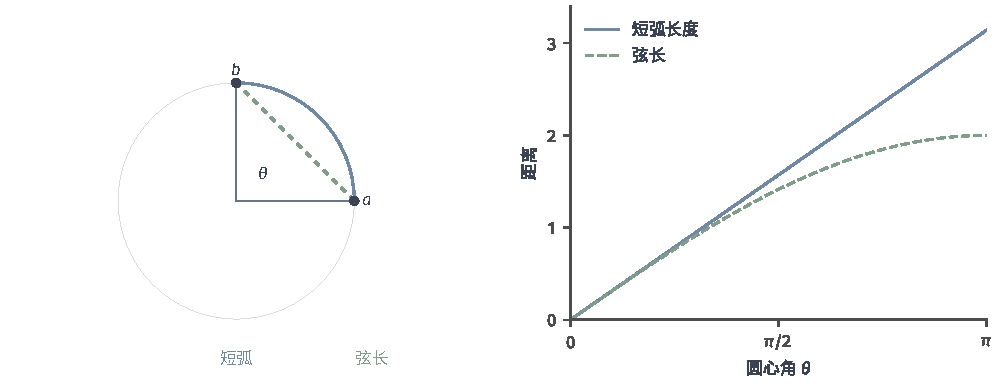
\includegraphics[width=169.0mm]{figures/00-shared/mathematical-preliminaries-upper/05-space-and-geometry/matplotlib/geometry-circle-distances/figure.pdf}
  \caption{完整单位圆的测地距离与环境弦长。左图夹角为$\pi/2$，
 蓝线为圆上的允许短弧，绿虚线为穿过圆内的环境线段；
 右图比较$\theta\in[0,\pi]$时的两种长度。完整圆允许选择两段弧中的较短者，
 不能与开中心线或二维开带的允许路径混用。图为解析教学示例。}
 \label{fig:geometry-circle-distances}
\end{figure*}

定义使用下确界是有意保留存在性问题。在穿孔平面
$\mathbb R^2\setminus\{\bm0\}$中，$(-1,0)^\top$与$(1,0)^\top$
之间可沿以被删原点为中心、半径任意小的半圆绕行，路径长度趋于$2$，
却没有长度恰为$2$的允许路径。空间始终只删去原点，变化的是绕行路径。
哪些全局条件保证达到下确界，将在固定端点的最短路径问题中讨论。

\subsection{对象的等价关系}
\label{sec:geometry-equivalence-relations}
\label{sec:geometry-symmetry-group-actions}

坐标可改变，不意味着任务输出必须不变。整体旋转点带时，长度不变，
表示朝向的向量却应同步旋转；重排点记录的行，则只改变编号而不移动空间中的点。
要准确规定这些要求，先明确允许哪些变换、如何复合，再指定它们作用于什么对象。

日常说的“旋转后结果不变”里，其实已经隐含了几条代数性质：
什么都不做也是一种变换；旋转后可以再旋回来；先转$\theta_1$再转$\theta_2$，
与一次转$\theta_1+\theta_2$相同。把“能接连做、也能撤销”的这些规则单独抽象出来，
就得到群。先有这套规则，才能严格表达“忽略旋转”或“随旋转同步变化”。

\begin{definition}[群]
\label{def:geometry-group}
\term{群}（group）$G$是带有二元运算的集合。运算封闭且满足结合律，
存在恒等元$e$，每个$g\in G$都存在逆元$g^{-1}$。
\end{definition}
群描述可以接连施加、也可以撤销的变换规则。集合中若只有若干增强操作，
复合后不再属于该集合，或者裁剪已丢失信息而不可逆，就还不能直接称其为群。
群的抽象乘法与对象上的实际操作，通过群作用联系。

\begin{definition}[群作用]
\label{def:geometry-group-action}
\term{群作用}（group action）是映射$G\times\mathcal X\to\mathcal X$，
记$(g,x)\mapsto g\cdot x$，满足
\begin{equation}
 e\cdot x=x,\qquad (g_1g_2)\cdot x=g_1\cdot(g_2\cdot x)
 \label{eq:geometry-group-action}
\end{equation}
对所有$x\in\mathcal X$和$g_1,g_2\in G$成立。
\end{definition}
第二条把群乘法解释为先做$g_2$、再做$g_1$。
同一个群可以作用在不同空间上，具体作用必须给出；讨论光滑流形上的作用时，
还要另行要求相应映射光滑。


如果任务确实要忽略某类变换，就应把该变换关联的输入视为等价。
\term{轨道}（orbit）$G\cdot x=\{g\cdot x:g\in G\}$收集从$x$出发能够得到的
所有输入。定义$x\sim y$当且仅当存在$g\in G$使$y=g\cdot x$，这是等价关系：
恒等元保证反身，逆元保证对称，复合保证传递。轨道的集合称为轨道商$\mathcal X/G$。
这时才有明确依据说两个不同记录代表同一个等价输入。


轨道商在这里只是等价类集合。即使原空间光滑，也不能直接宣布商仍是同维或更低维
的光滑流形。例如平面上全部旋转组成的群$\mathrm{SO}(2)$作用于$\mathbb R^2$，
轨道按半径标记，
商可识别为$[0,\infty)$：原点的轨道只有一个点，其余轨道是圆。
商的端点不满足无边界一维流形的局部开区间条件。若讨论一般商的光滑结构，
需要补充作用的正则性条件，不能仅凭“去掉一个旋转自由度”作维数相减。

图~\ref{fig:vol1-add-geometry-rotation-orbits}显示半径为何能给旋转轨道编号。同一圆上的点经旋转互相到达，而原点始终不动；原点轨道的特殊性使商的端点不能被当作普通内部点。
\begin{figure}[!htb]
  \centering
  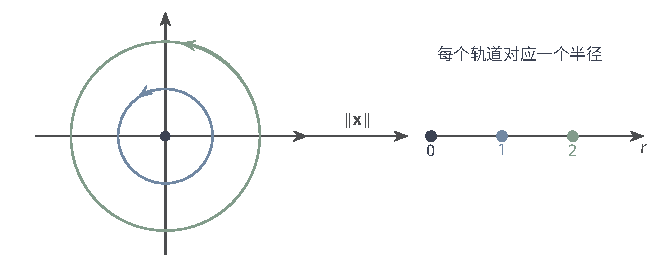
\includegraphics[width=112mm]{figures/00-shared/mathematical-preliminaries-upper/05-space-and-geometry/tikz/comprehension-additions/geometry-rotation-orbits.pdf}
  \caption{旋转轨道与半径商。$\mathrm{SO}(2)$作用于平面时，半径为$1$、$2$的圆分别形成一条轨道，原点单独形成一条轨道。右侧用$r=\lVert \bm x\rVert_2\geq0$记录轨道；圆上的不同位置被归为同一点，半径不同的圆仍分开。}
  \label{fig:vol1-add-geometry-rotation-orbits}
\end{figure}



\subsubsection{比例等价下的射影表示}
\label{sec:geometry-projective-representation}

若一条观测只确定方向，$(2,1)^\top$与$(4,2)^\top$应表示同一对象，
零向量却没有方向。前面的轨道商允许精确表达这种忽略尺度的规则：
在$\mathbb R^{n+1}\setminus\{\bm0\}$上令
$\bm x\sim\bm y$当且仅当$\bm y=\lambda\bm x$，其中$\lambda\ne0$。
等价类组成\term{实射影空间}（real projective space）$\mathbb{RP}^n$，
用\term{齐次坐标}（homogeneous coordinates）
$[\bm x]=[x_1:\cdots:x_{n+1}]$记录一个等价类。
坐标数是$n+1$，但共同倍数被忽略；它不同于上一章按加法子空间取商的线性空间。

等价类集合还没有自动带上流形结构。为给它一个具体的环境，
把$[\bm x]$记录为对称矩阵
\[
 \bm P(\bm x)=\frac{\bm x\bm x^\top}{\bm x^\top\bm x}.
\]
它是向直线$\operatorname{span}\{\bm x\}$的正交投影，满足
$\bm P^2=\bm P$、$\operatorname{tr}\bm P=1$。
两个非零向量给出相同投影，当且仅当它们成比例。
因此可以将射影点视为对称矩阵欧氏环境中的这些秩一投影，采用诱导的邻域与开集。
不同投影可用互不相交的小矩阵球区分；下面有限张仿射图又各有由有理球产生的可数基。
这排除了只靠光滑过渡拼接、却没有可分离邻域或可数基的情况。
它也给出通常的比例商拓扑：将代表缩到单位球面后，$\bm P$连续且只合并互为相反数的点；
球面中由完整对跖点对组成的闭集是紧集，其矩阵像仍紧而闭，
故商的开闭集与这里的诱导拓扑一致。

\paragraph{仿射图与无穷远位置}
要把比例记录变成普通坐标，先选一个非零分量。例如在$x_{n+1}\ne0$的范围内，
每个类都唯一写成$[u_1:\cdots:u_n:1]$，其中$u_i=x_i/x_{n+1}$。
这是一张取值于$\mathbb R^n$的\term{仿射图}（affine chart）。
改选$x_j\ne0$也得到一张图；重叠范围内的转换只是坐标之比，分母非零时光滑，
还可在矩阵环境中核对这些图：$x_j\ne0$恰对应$P_{j,j}>0$，
坐标由$x_i/x_j=P_{i,j}/P_{j,j}$恢复。
该恢复式在相应环境开集上光滑；反向将第$j$分量设为$1$再代入$\bm P$，也得到光滑参数化。
恢复映射与参数化复合为恒等，因而参数化的微分满列秩。
这就符合前面欧氏嵌入型流形的定义，得到$n$维光滑流形，
而不只是一个带光滑坐标转换公式的等价类集合。
相对于选定的最后分量图，$x_{n+1}=0$的类称为\term{无穷远点}（point at infinity）。
它不是向坐标中加入数值$\infty$，而是本图未覆盖、可在其他图中正常记录的方向。
例如射影直线上$[2:4]=[1:2]$在末分量图的坐标为$1/2$，
$[1:0]$不在这张图中，却在首分量图中有坐标$0$。

在射影平面中，非零系数向量$\bm\ell=(a,b,c)^\top$表示直线
$\bm\ell^\top\bm x=0$，系数的共同非零倍数仍表示同一直线。
在$x_3=1$的图中这就是$au+bv+c=0$。
若要从两点构造直线，只需找与两点都正交的系数。
对$\bm x,\bm y\in\mathbb R^3$，定义叉积
\[
 \bm x\times\bm y=
 (x_2y_3-x_3y_2,\ x_3y_1-x_1y_3,\ x_1y_2-x_2y_1)^\top.
\]
两点不成比例时$\bm\ell=\bm x\times\bm y\ne0$，满足所需的两个线性方程；
反过来，两条不同直线的交点由$[\bm\ell_1\times\bm\ell_2]$给出。
例如平行直线$u=0$与$u=1$的系数为$(1,0,0)^\top$、$(1,0,-1)^\top$，
叉积为$(0,1,0)^\top$，即它们在这张仿射图之外的共同方向。
若两点或两线本来相同，叉积为零，不能把零向量当成一个射影点。

\paragraph{坐标变换下的点线对应}
给定可逆$(n+1)$阶矩阵$\bm H$，映射
$[\bm x]\mapsto[\bm H\bm x]$称为\term{射影变换}（projective transformation）。
它不依赖代表元，因为输入缩放只使输出同步缩放；$\bm H$乘非零常数也不改变变换。
平面中若$\bm x'=\bm H\bm x$，则直线系数按
$\bm\ell'=\bm H^{-\top}\bm\ell$变化，
从而$\bm\ell'^\top\bm x'=\bm\ell^\top\bm x$，点在线上的关系被保留。
这不保证欧氏长度、角度或平行性被保留。
仿射变换是底行为$(0,\ldots,0,1)$的特别情形，保持选定的无穷远超平面；
一般射影变换则可能把有限点送到该图的无穷远处。

例如
\[
 \bm H=\begin{bmatrix}1&0&0\\0&1&0\\1&0&1\end{bmatrix},
 \qquad (u,v)\longmapsto
 \left(\frac{u}{u+1},\frac{v}{u+1}\right)
 \quad (u\ne-1).
\]
$u=-1$上的点仍有合法齐次像，只是不能在输出末分量图中做透视除法。
这个例子解释了为什么除以最后一个分量必须检查非零，而不能把该除法当成全局线性映射。

\paragraph{由点对应估计平面变换}
当$\bm H$未知，给定有限点$(u_i,v_i)$及其对应$(u'_i,v'_i)$，
要找一个共同射影变换解释这些对应。令$\bm x_i=(u_i,v_i,1)^\top$，
$\bm x'_i=(u'_i,v'_i,1)^\top$，比例关系可消去未知尺度，写成
$\bm x'_i\times(\bm H\bm x_i)=\bm0$。
三条分量方程中只有两条独立。将$\bm H$的元素按行排为
$\bm h=(h_{1,1},h_{1,2},h_{1,3},h_{2,1},\ldots,h_{3,3})^\top$，可取
\begin{equation}
 \begin{bmatrix}
 u_i&v_i&1&0&0&0&-u'_i u_i&-u'_i v_i&-u'_i\\
 0&0&0&u_i&v_i&1&-v'_i u_i&-v'_i v_i&-v'_i
 \end{bmatrix}\bm h=\bm0.
 \label{eq:geometry-planar-dlt}
\end{equation}
这里的按行排列已显式规定，不是上一章默认按列的$\operatorname{vec}$。
把对应点的两行堆叠为$\bm A$，就在$\|\bm h\|_2=1$下最小化
$\|\bm A\bm h\|_2$，回用上一章的齐次最小二乘。
这种先消去比例再线性估计的做法称为\term{直接线性变换法}
（direct linear transformation, DLT）\scite{vision-hartley-zisserman2004}。
它给出代数误差准则下的估计；若要最小化原坐标的几何距离，还需另外规定并求解该目标。
含噪声的最弱奇异向量也未必还原成可逆矩阵，因此还须检查估计是否退化，
不能只因线性子问题返回了一个向量便认为已得到合法射影变换。

一个可逆三阶矩阵有九个参数，忽略共同尺度后有八个自由度。
四对点在一般位置时可以确定一个变换：这里一般位置要求两组各自都没有三点共线。
理由是前三点可选为齐次基，第四点在这组基中的三个系数均非零；
用列尺度把第四点调为三个基向量之和后，两组构成相同的四点框架，变换便唯一到共同倍数。
因此理想数据的$\bm A$秩为八，零空间给出所需比例；
点数够而点共线时，计数并不能排除退化。
上面的$\bm H$把$(0,0),(1,0),(0,1),(1,1)$依次映为
$(0,0),(1/2,0),(0,1),(1/2,1/2)$，代入八行方程均为零，
其九维参数向量除以$2$后满足单位范数约束。

实际坐标可能有很大的平移量或不同数量级，直接组装二次坐标乘积会使计算失衡。
可以先将每组点移到其均值为零，再缩放使到原点的平均欧氏距离为$\sqrt2$。
记这两个可逆仿射矩阵为$\bm T,\bm T'$，在归一化坐标中估计$\widetilde{\bm H}$后，
由$\widetilde{\bm H}=\bm T'\bm H\bm T^{-1}$恢复
$\bm H=\bm T'^{-1}\widetilde{\bm H}\bm T$。
若平均距离为零，数据本身已退化，不能继续做这一缩放。
归一化常改善数值平衡，但也选择了代数残差的尺度；
上一章已经说明，它不保证含噪问题的几何误差目标保持不变。

\section{运算与映射}
\label{sec:geometry-operations}

位置映射将一个点送到另一个点或一组特征，映射的叠加与复合组织多步作用。
点一旦变化，还需说明速度怎样传递、旧方向怎样搬到新位置，以及怎样从切向步产生可行的新点。
最后再从度量计算区域体积，为下一章的函数积分提供几何权重。
位置更新先建立一般测地、指数与回缩，再用三维旋转说明约束如何具体落实到矩阵和四元数，
并区分单步更新与给定两次朝向的最短弧插值。它们回答不同的输入输出问题，
共同要求产生的新位置仍在指定空间中。

\subsection{空间之间的映射}
\label{sec:geometry-point-maps}

圆上位置可以映到横坐标，也可以映到另一个曲面上的位置。
要判断这样的映射是否光滑，先把两端位置都转成局部欧氏坐标。
设$F:\mathcal M\to\mathcal N$，用输入参数化$\varphi$与输出参数化$\psi$
记录后，$\psi^{-1}\circ F\circ\varphi$是欧氏开集之间的映射。
若所有适用图中的表达都光滑，就称$F$光滑；光滑过渡和链式法则保证换图不改变这个判断。
输出也可以是$\mathbb R^r$中的特征，而不一定是另一个弯曲空间中的位置。
例如单位圆上的$(x,y)\mapsto x$读取环境横坐标，仍是合法的光滑映射。

\subsection{映射的叠加}
\label{sec:geometry-map-addition}

映射叠加要求各分支具有共同定义域，输出落在同一个可加的线性空间。
若$F_j:\mathcal M\to V$、$a_j$固定，则
$F(p)=\sum_j a_jF_j(p)$定义新的映射；各分支光滑时，坐标表达逐项相加仍光滑。
这里不要求$\mathcal M=V$。若输出是球面位置，直接相加通常不再可行；
若另作归一化，还须排除和为零，并把归一化看作新的复合步骤。

点云分支可以各自接收整幅点云，再把同形特征相加；共享逐点分支也可以先产生
各点特征，再求和汇聚。两者的输入对象不同，不能仅凭代码中都有求和就视为同一个作用。

\subsection{映射的复合}
\label{sec:geometry-map-composition}
\label{sec:geometry-group-invariance-equivariance}


当$F:\mathcal M\to\mathcal N$、$H:\mathcal N\to\mathcal P$的中间对象匹配时，
$(H\circ F)(p)=H(F(p))$。下面用复合表达变换后的响应。
把输入按$g$改变之后再求$F$，输出会有两种可能的反应：一种是不变，即输出值与
未改变输入时相同，这称为不变性；另一种是按某个已知方式跟着改变，例如输入旋转
多少度、输出也跟着旋转多少度，这称为等变性。前者可以理解为“任务答案不受该变换
影响”，后者则是“答案随该变换同步变化”。两种要求都要指明作用在哪个对象上，
不能只写“对变换稳定”。
当对象是向量且作用保持线性组合时，可以直接用线性代数描述响应。
\begin{definition}[线性表示]
\label{def:geometry-linear-representation}
\term{线性表示}（linear representation）是映射
$\rho:G\to\operatorname{GL}(V)$，满足
\begin{equation}
 \rho(e)=\bm I,\qquad \rho(g_1g_2)=\rho(g_1)\rho(g_2),
 \label{eq:geometry-linear-representation}
\end{equation}
其中$\operatorname{GL}(V)$是向量空间$V$上全部可逆线性算子组成的群。
\end{definition}
它用线性算子实现群的复合规则，因而$\rho$把一个群变换对应成一组矩阵运算。
输入与输出可以取不同表示，这正好用来区分上述两种反应：若输入平面坐标按旋转矩阵
$\bm R(\theta)$变换，则标量输出“不变”对应$\rho(g)=1$；方向向量输出“同步旋转”
对应$\rho(g)=\bm R(\theta)$。同一个$g$在两处对应不同矩阵，并不矛盾，
因为它们作用在不同的空间上。

平面旋转群$\mathrm{SO}(2)$由行列式为$1$的二维正交矩阵组成。
角度$\theta$对应
\begin{equation}
 \bm R(\theta)=
 \begin{bmatrix}\cos\theta&-\sin\theta\\\sin\theta&\cos\theta\end{bmatrix},
 \qquad
 \bm R(\theta_1)\bm R(\theta_2)=\bm R(\theta_1+\theta_2).
 \label{eq:geometry-planar-rotation-group}
\end{equation}
同一旋转可作用于一个点、整组点，或通过改变自变量作用于图像函数。
这些输入空间不同。对点带整体旋转时，坐标写成$\bm R(\theta)\Phi(s,u)$，
局部参数$(s,u)$可以不变；这是环境表示改变，并非必须重新定义内部位置。

有限集合$\{1,\ldots,n\}$的全部置换组成对称群$S_n$。
约定置换矩阵满足$(\bm P_\pi\bm X)_{i,:}=\bm X_{\pi^{-1}(i),:}$，
则$\bm P_{\pi_1\pi_2}=\bm P_{\pi_1}\bm P_{\pi_2}$。
对点云$\bm X\in\mathbb R^{n\times D}$，行置换改变记录顺序，
而$D$维旋转矩阵$\bm R$作用在坐标列上，写为$\bm X\bm R^\top$。矩阵乘法的外形相似，
实际被改变的对象和索引却不同。


\begin{definition}[不变映射]
\label{def:geometry-invariant-map}
群$G$作用于$\mathcal X$。映射$f:\mathcal X\to\mathcal Y$若满足
\begin{equation}
 f(g\cdot x)=f(x)\qquad(g\in G,\ x\in\mathcal X),
 \label{eq:geometry-invariant-map}
\end{equation}
称为对该作用\term{不变}（invariant）。
\end{definition}
不变映射在同一轨道上取相同值，因此可写成
$f=\widetilde f\circ\pi$，其中$\pi(x)=G\cdot x$是商映射。
令$\widetilde f(G\cdot x)=f(x)$之所以不依赖代表元，正是由不变性保证。
但$f$也可能把不同轨道映到同一输出；不变不等于保留了区分轨道的全部信息。


当输出必须保留位置或朝向时，合理要求是让它按约定同步变化。
\begin{definition}[等变映射]
\label{def:geometry-equivariant-map}
若$G$还作用于$\mathcal Y$，把输出作用记为$\rho(g)$，映射
$F:\mathcal X\to\mathcal Y$满足
\begin{equation}
 F(g\cdot x)=\rho(g)F(x)\qquad(g\in G,\ x\in\mathcal X),
 \label{eq:geometry-equivariant-map}
\end{equation}
则称为\term{等变}（equivariant）。输出作用不必线性；当$\mathcal Y$是向量空间
且$\rho$为线性表示时，右端才是相应线性算子的作用。
\end{definition}
例如预测点带朝向时，输入旋转后，输出向量也应旋转。
标量类别、位置坐标和分割掩码所需的响应不同，不变性不是比等变性更好的统一目标。
等变映射之后接不变汇总可得到不变输出；反过来，已丢弃朝向的信息通常不能恢复。

图~\ref{fig:vol1-add-geometry-invariant-equivariant}沿用同一次平面旋转，把标量读取与向量映射并排核对。判断响应时，要同时看清变换的是哪个平面向量，以及任务要保留长度还是朝向。
\begin{figure}[!htb]
  \centering
  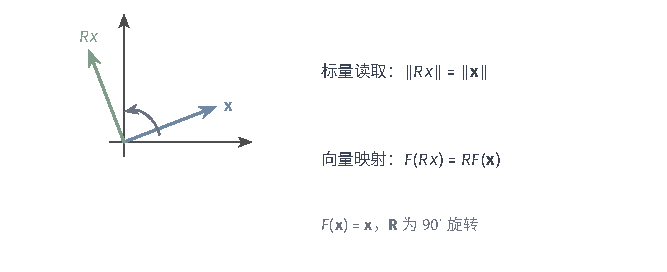
\includegraphics[width=112mm]{figures/00-shared/mathematical-preliminaries-upper/05-space-and-geometry/tikz/comprehension-additions/geometry-invariant-equivariant.pdf}
  \caption{同一旋转下的两种响应。蓝向量$\bm x=(1.3,0.5)^\top$逆时针转$90^\circ$成为绿向量$Rx=(-0.5,1.3)^\top$。标量长度读取满足$\lVert Rx\rVert_2=\lVert \bm x\rVert_2$，所以不变；恒等映射$F(\bm x)=\bm x$满足$F(Rx)=RF(\bm x)$，所以向量输出等变。}
  \label{fig:vol1-add-geometry-invariant-equivariant}
\end{figure}



在点云上，对每行使用同一个映射$\phi$，令
$F(\bm X)_{i,:}=\phi(\bm X_{i,:})$，则第$i$行直接给出
\[
 F(\bm P_\pi\bm X)_{i,:}
 =\phi(\bm X_{\pi^{-1}(i),:})
 =(\bm P_\pi F(\bm X))_{i,:}.
\]
所以逐点共享映射对行置换等变。再对行求和，
$f(\bm X)=\sum_i\phi(\bm X_{i,:})$，重编号只改变求和次序，因而不变。
这证明了响应关系，尚未证明求和表示能够区分任务需要的全部点集。

平移作用的例子需要同时规定定义域。对全空间上的可积函数
$k,f\in L^1(\mathbb R^d)$，这里$L^1$表示绝对值积分有限的函数。
令$(T_{\bm a}f)(\bm x)=f(\bm x-\bm a)$，
卷积是将一个函数平移后与另一个相乘并积分：
\begin{align}
 (k*(T_{\bm a}f))(\bm x)
 &=\int_{\mathbb R^d}k(\bm x-\bm y)f(\bm y-\bm a)\,\mathrm d\bm y\\
 &=\int_{\mathbb R^d}k(\bm x-\bm a-\bm z)f(\bm z)\,\mathrm d\bm z
   =(T_{\bm a}(k*f))(\bm x).
 \label{eq:geometry-translation-convolution-equivariance}
\end{align}
变量替换$\bm z=\bm y-\bm a$说明卷积与平移可交换。
$L^1$条件使等式几乎处处成立，即除去一个Lebesgue零测集后成立。
若积分处处绝对收敛，例如一个函数连续有界、
另一个可积，就可以逐点理解。有限图像的零填充、裁剪和下采样可能破坏所声称的
平移等变性；循环平移配周期边界和只比较有效区域又是另外的作用，须逐项核对。

\begin{table*}[htbp]
 \centering\small
 \begin{tabularx}{\linewidth}{@{}lXX@{}}
 \toprule
 输入作用 & 不变输出 & 等变输出及其作用\\
 \midrule
 平面旋转$\bm x\mapsto\bm R\bm x$
 & $\lVert\bm x\rVert_2$ & $F(\bm x)=\bm x$，输出也乘$\bm R$\\
 点记录行置换$\bm X\mapsto\bm P\bm X$
 & 逐行映射后求和 & 逐行共享映射，输出行也乘$\bm P$\\
 全空间信号平移
 & 可积函数的全空间积分 & 与固定可积核卷积，输出信号同样平移\\
 \bottomrule
 \end{tabularx}
 \caption{先指定输入与输出作用，才能判断不变或等变。全空间信号的恒等式不自动适用于
 有裁剪、边界填充或下采样的有限窗口；结构响应也不保证表示保留了任务所需的全部信息。}
 \label{tab:geometry-invariance-equivariance}
\end{table*}
表~\ref{tab:geometry-invariance-equivariance}把同一个输入作用的两种输出要求并列，
区别在于输出应该忽略变换，还是记录变换后的对象。


群复合还可以构造相对位置表示。对实数位置$t$和频率$\omega$，
令$\bm R_\omega(t)=\bm R(\omega t)$。同时平移位置$s,t$不改变$t-s$，而旋转复合给出
\begin{equation}
 \bm R_\omega(s)^\top\bm R_\omega(t)=\bm R_\omega(t-s).
 \label{eq:geometry-rotary-relative-position}
\end{equation}
所以对固定二维向量$\bm q,\bm k$，
\begin{equation}
 (\bm R_\omega(s)\bm q)^\top(\bm R_\omega(t)\bm k)
 =\bm q^\top\bm R_\omega(t-s)\bm k.
 \label{eq:geometry-rotary-dot-product}
\end{equation}
多个频率块并置仍保留这一恒等式，位置引入的旋转因子只通过相对位移出现。
这不意味着整个注意力网络只依赖相对位置：$\bm q,\bm k$的生成、其他位置特征、
偏置、窗口与边界仍可能含绝对位置信息。单个非零频率块的周期为$2\pi/|\omega|$，
多频率组合的可区分范围需连同频率、数值精度和序列长度分析，不能据此承诺无限长度
无碰撞。这里比较的是指定代数变换；后文沿曲面搬运方向还要给出路径和联络，
不能把两种操作都简化为一次任意旋转。


\subsection{切向量的映射}
\label{sec:geometry-tangent-maps}

例如圆上的点在移动时，其横坐标也随之变化；给定点的瞬时速度，就应能计算读数的瞬时变化。
因此，除了点映射本身，还要建立它对切向速度的作用。
对第\ref{sec:geometry-point-maps}节定义的光滑映射$F:\mathcal M\to\mathcal N$，
取输入、输出两端的局部参数化$\varphi,\psi$。
它在$\bm p$处的微分（differential）把输入速度转成输出速度：
\[
 \mathrm dF_{\bm p}(\bm v)
 =\left.\frac{\mathrm d}{\mathrm dt}F(\gamma(t))\right|_{t=0},
 \qquad\gamma(0)=\bm p,\quad\gamma'(0)=\bm v.
\]
若$\bm v=\bm J_\varphi(\bm z)\bm a$，令
$\bm w=\psi^{-1}(F(\bm p))$，则
\begin{equation}
 \mathrm dF_{\bm p}(\bm v)
 =\bm J_\psi(\bm w)
   \bm J_{\psi^{-1}\circ F\circ\varphi}(\bm z)\bm a.
 \label{eq:geometry-map-differential}
\end{equation}
右端只依赖初速度，不依赖实现速度的曲线，因此定义良好且线性。
坐标变换时两侧的Jacobian因链式法则相互抵消；
$\mathrm dF_{\bm p}:T_{\bm p}\mathcal M\to T_{F(\bm p)}\mathcal N$
是几何映射，矩阵只是其坐标记录。复合还满足
$\mathrm d(H\circ F)_{\bm p}=\mathrm dH_{F(\bm p)}\circ\mathrm dF_{\bm p}$。

对标量函数$f:\mathcal M\to\mathbb R$，微分读取速度引起的一阶数值变化。
\term{余切空间}（cotangent space）$T_{\bm p}^*\mathcal M$就是
$T_{\bm p}\mathcal M$的线性泛函空间，泛函的含义沿用
\BookSectionRef{sec:linear-algebra-scalar-readouts}{第\ref{sec:linear-algebra-scalar-readouts}节}的有限维标量读取。
有限维向量空间上的全部线性读取组成其对偶空间（dual space）；
所以$\mathrm df_{\bm p}\in T_{\bm p}^*\mathcal M$，不是一个切向量。
沿用前面的局部坐标$(z^1,\ldots,z^d)$与坐标切基$\partial_i$，
其对偶基$\mathrm dz^i$满足$\mathrm dz^i(\partial_j)=\delta_{i,j}$，
也就是$\mathrm dz^i(\sum_j a^j\partial_j)=a^i$：它读出速度的第$i$个坐标系数。于是
\[
 \mathrm df=\sum_i\partial_i(f\circ\varphi)\,\mathrm dz^i,\qquad
 \mathrm df\!\left(\sum_i a^i\partial_i\right)
 =\sum_i\partial_i(f\circ\varphi)a^i.
\]
例如圆上$f(\cos\theta,\sin\theta)=\cos\theta$，
角速度$a$对应的数值变化为$-a\sin\theta$。

在图~\ref{fig:vol1-add-geometry-differential-readout}中，圆上的速度向量指向左上方，而横坐标读数只保留其中向左的变化率。一个切向速度经过微分读取后成为标量，二者的对象类型因此不同。
\begin{figure}[!htb]
  \centering
  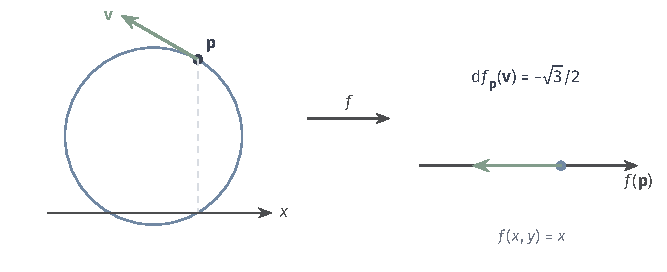
\includegraphics[width=112mm]{figures/00-shared/mathematical-preliminaries-upper/05-space-and-geometry/tikz/comprehension-additions/geometry-differential-readout.pdf}
  \caption{微分读取速度产生的数值变化。单位圆上取$\theta=\pi/3$，$\bm p=(1/2,\sqrt3/2)$，单位角速度给出$\bm v=(-\sqrt3/2,1/2)$。函数$f(x,y)=x$把点送到横坐标，微分给$\mathrm df_{\bm p}(\bm v)=-\sqrt3/2$。绿色箭头表示速度或变化率的方向；两侧箭头不共用长度比例。}
  \label{fig:vol1-add-geometry-differential-readout}
\end{figure}


要把这个线性读取规则表示成“最陡方向”，还须指定方向长度，
第\ref{sec:geometry-point-optimization}节将用已经建立的度量，把这个读取规则表示为梯度。

\subsection{切向量的搬运}
\label{sec:geometry-tangent-transport}
\label{sec:geometry-connection-comparison}
\label{sec:geometry-riemannian-curvature}

\label{sec:geometry-cross-point-comparison-curvature}
\label{sec:geometry-parallel-transport}

沿路径计算长度时，每个位置只输出一个标量。若要问速度有没有转弯，
或相邻两点的方向是否一致，就必须比较不同切空间中的向量。
即使流形嵌在同一个欧氏空间内，直接相减也可能产生法向分量：
圆上恒速运动的速度导数指向圆心，却没有沿圆加速。
需要把环境变化与流形内的方向变化分开。下面建立联络、平行移动和曲率，
所用的Riemann几何基础可参见Lee的教材\scite{math-lee2018riemannian}。

先用单位圆上的一个具体比较说明困难在哪里。在$\bm p=(1,0)^\top$处的切向量
$\bm u=(0,1)^\top$与在$\bm q=(0,1)^\top$处的切向量$\bm w=(-1,0)^\top$
都表示“沿圆逆时针前进”，直觉上应当判为同一个方向。
但作为$\mathbb R^2$中的向量，$\bm u-\bm w=(1,1)^\top$并不为零，
其长度是$\sqrt2$；若据此认为两者相差很大，就把两个不同切空间中的向量当成同一空间中的对象了。
更麻烦的是$\bm u$本身并不属于$T_{\bm q}\mathbb S^1$：
在$\bm q$处，切空间是水平的，$\bm u$却指向竖直方向。
所以在曲面上谈“方向有没有改变”“两个点的朝向是否一致”，
必须额外规定一个把$T_{\bm p}\mathcal M$中的向量搬到$T_{\bm q}\mathcal M$的规则。
这个规则不能随便取：它要与度量相容，否则“长度不变”这句话就失去依据；
还要沿路径一致地定义，否则搬运结果会依赖人为的分段方式。
联络正是满足这些要求的规则，平行移动是它给出的搬运结果。


把圆周上的单位切向速度画在每个位置，得到一个向量场。
沿圆周求它的环境导数会出现法向分量，但流形内的方向变化应仍是切向的。
下面用联络规定这种微分：它保持切向性，也保留求导对加法与函数乘积的规则。
联络据此比较邻近位置的方向，无须把所有切空间认作同一个固定子空间。

\begin{definition}[向量场与联络]
\label{def:geometry-connection}
光滑\term{向量场}（vector field）$\bm V$在每个$\bm p\in\mathcal M$选取
$\bm V(\bm p)\in T_{\bm p}\mathcal M$，其坐标分量光滑。
\term{联络}（connection）为两个光滑向量场$\bm U,\bm V$指定向量场
$\nabla_{\bm U}\bm V$，称为$\bm V$沿$\bm U$的
\term{协变导数}（covariant derivative），并满足
\[
 \begin{aligned}
 \nabla_{f\bm U+h\bm W}\bm V
   &=f\nabla_{\bm U}\bm V+h\nabla_{\bm W}\bm V,\\
 \nabla_{\bm U}(a\bm V+b\bm W)
   &=a\nabla_{\bm U}\bm V+b\nabla_{\bm U}\bm W,\\
 \nabla_{\bm U}(f\bm V)
   &=\bm U(f)\bm V+f\nabla_{\bm U}\bm V.
 \end{aligned}
\]
其中$f,h$为光滑函数，$a,b\in\mathbb R$，
$\bm U(f)=\mathrm df(\bm U)$为方向导数。
\end{definition}
第一项对求导方向按光滑函数线性，第二项对被求导对象按常数线性，
第三项则说明不能把第二项也加强为按光滑函数线性：
系数本身的变化必须保留。欧氏空间的普通方向导数满足这三项规则；
一般流形上，单独求坐标分量的导数不够，因为坐标切基本身也在变。

后一点值得用最普通的经验体会。在一张直角坐标纸上，沿水平网格移动时，
网格本身不动，箭头方向是否改变只需看它的分量怎么变。
换到一张随位置弯曲、伸缩的坐标网，哪怕箭头在几何上完全没动，
它在网格中的分量也会变化——因为网格线本身在转、在变。
反过来，分量不变也可能表示箭头其实跟着网格一起转了。
联络要扣除的正是这种“尺子和网格在动”造成的虚假变化，
所以不能只对坐标分量求普通导数。

度量已经规定长度，新的导数应当与这一判断相容。
此外，非坐标方向场先后作用的顺序本来就可能不同，不能把这种差异误认为额外的几何扭转。
定义交换子$[\bm U,\bm V]$为对任意光滑$f$满足
\[
 [\bm U,\bm V](f)=\bm U(\bm V(f))-\bm V(\bm U(f))
\]
的向量场；在坐标基下，其第$k$个分量为
$\sum_i(U^i\partial_iV^k-V^i\partial_iU^k)$。
坐标方向$\partial_i,\partial_j$的交换子为零，一般方向场则未必。

\begin{example}[平面上不可交换的方向场]
\label{ex:geometry-plane-field-commutator}
在欧氏平面取$\bm U=\partial_x$、$\bm V=x\partial_y$。
$\bm U$始终沿$x$轴，$\bm V$沿$y$轴但其大小随$x$改变。
对任意光滑函数$f$，
\[
 \bm U(\bm V(f))=\partial_yf+x\partial_x\partial_yf,\qquad
 \bm V(\bm U(f))=x\partial_y\partial_xf,
\]
故$[\bm U,\bm V]=\partial_y$。先沿$x$方向移动，会改变随后沿$\bm V$移动的速度；
两个方向场的顺序差异在平面上就会出现。
欧氏空间的普通方向导数还给出
\[
 \nabla_{\bm U}\bm V=\partial_y,\qquad
 \nabla_{\bm V}\bm U=\bm0.
\]
二者之差恰是交换子。这个平坦例子说明，方向场本身随位置变化所产生的差异，
需要与几何结构额外产生的差异分开。
\end{example}

\begin{definition}[Levi--Civita联络]
\label{def:geometry-levi-civita-connection}
给定Riemann度量$g$，同时满足下列度量相容与无挠条件的联络，
称为它的\term{Levi--Civita联络}（Levi--Civita connection）：
\begin{align*}
 \bm U\bigl(g(\bm V,\bm W)\bigr)
 &=g(\nabla_{\bm U}\bm V,\bm W)+g(\bm V,\nabla_{\bm U}\bm W),\\
 \nabla_{\bm U}\bm V-\nabla_{\bm V}\bm U&=[\bm U,\bm V].
\end{align*}
\end{definition}
度量相容使内积的求导仍满足乘积法则；无挠规定联络在交换两个方向场时，
不产生交换子之外的差异。无挠\emph{不}声称
$\nabla_{\bm U}\nabla_{\bm V}\bm W
=\nabla_{\bm V}\nabla_{\bm U}\bm W$，后者涉及本节末尾的曲率。

每个光滑Riemann度量唯一确定这样的联络。其唯一性可以从两项条件直接看出：
轮换$\bm U,\bm V,\bm W$的度量相容等式，并用无挠条件消去交换项，得到
\begin{align}
 2g(\nabla_{\bm U}\bm V,\bm W)
 &=\bm U g(\bm V,\bm W)+\bm V g(\bm W,\bm U)
   -\bm W g(\bm U,\bm V)\notag\\
 &\quad+g([\bm U,\bm V],\bm W)-g([\bm V,\bm W],\bm U)
   +g([\bm W,\bm U],\bm V).
 \label{eq:geometry-koszul-formula}
\end{align}
右端只含已知度量、向量场和普通方向导数，故已有联络至多只有一个。
要由此构造联络，还需确认右端确实是对$\bm W$的逐点线性读取。
记右端为$K(\bm U,\bm V,\bm W)$。把$h\bm W$代入时，
乘积法则产生的$\bm U(h)$、$\bm V(h)$项分别与交换子中的项抵消，
所以$K(\bm U,\bm V,h\bm W)=hK(\bm U,\bm V,\bm W)$；加法线性也成立。
在局部基中，这意味着它只读取$\bm W$在当前点的值。
正定内积于是把$K/2$唯一表示成向量；其分量由光滑矩阵$\bm G^{-1}$乘光滑读数组成，
所以得到光滑向量场。

同样展开前两个变量，得到
\[
\begin{aligned}
 K(h\bm U,\bm V,\bm W)&=hK(\bm U,\bm V,\bm W),\\
 K(\bm U,h\bm V,\bm W)&=hK(\bm U,\bm V,\bm W)
   +2\bm U(h)g(\bm V,\bm W).
\end{aligned}
\]
结合常数线性，恰好给出联络的三条求导规则。
在公式中交换第二、第三个向量场，再将两式相加，
得到$2\bm U g(\bm V,\bm W)$，即度量相容；交换前两个变量后相减，
得到$2g([\bm U,\bm V],\bm W)$，即无挠。这样才完成存在性构造。
实际计算通常使用坐标系数或环境投影。

对继承欧氏度量的嵌入流形，设$\bm P_{\bm p}$为环境空间到
$T_{\bm p}\mathcal M$的正交投影，则
\begin{equation}
 \nabla_{\bm U}\bm V(\bm p)
 =\bm P_{\bm p}\,\mathrm d\bm V_{\bm p}(\bm U(\bm p)).
 \label{eq:geometry-projected-connection}
\end{equation}
这里把$\bm V$视为取值于环境$\mathbb R^D$的映射，先求环境导数再投影。
投影保持对切向量的内积，所以欧氏内积的乘积法则给出度量相容；
环境方向导数之差是已经切向的交换子，投影后仍不变，故也无挠。
由唯一性，这正是诱导度量的Levi--Civita联络。
若度量不是环境诱导度量，不能继续沿用这个欧氏正交投影公式。


现在固定路径$\gamma(t)$和起点切向量，希望沿路保持方向。
“保持”不是要求环境坐标分量不变，而是要求联络测得的变化为零。
在坐标基中写
$\nabla_{\partial_i}\partial_j=\sum_k\Gamma^k_{i,j}\partial_k$。
这些系数称为Christoffel符号，记录坐标切基随位置的变化；第\ref{sec:geometry-position-updates}节将从度量求出其表达式。

\begin{example}[坐标基变化怎样进入导数]
\label{ex:geometry-coordinate-connection}
正半轴采用欧氏度量，在坐标$x>0$中，基向量$\partial_x$处处相同，故
$\nabla_{\partial_x}\partial_x=0$。改用$x=e^u$记录同一位置，则
$\partial_u=e^u\partial_x$随$u$改变；按环境求导得到
$\nabla_{\partial_u}\partial_u=e^u\partial_x=\partial_u$，所以
$\Gamma^u_{u,u}=1$，而$\Gamma^x_{x,x}=0$。
同一个环境常向量场$\bm V=\partial_x$在新基中的分量为$V^u=e^{-u}$。
只求分量导数会得到$-e^{-u}$，还需计入基向量变化：
\[
 \nabla_{\partial_u}\bm V
 =\left(\frac{\mathrm d V^u}{\mathrm du}
               +\Gamma^u_{u,u}V^u\right)\partial_u
 =(-e^{-u}+e^{-u})\partial_u=0.
\]
这项修正使同一个常向量场在两种坐标中都被判为没有变化。
\end{example}

对于一般路径，还要乘上各坐标方向的运动速度，才能把这些基变化沿路径累加。
沿$\gamma(t)=\varphi(\bm z(t))$的向量
$\bm V(t)=\sum_jV^j(t)\partial_j$满足
\begin{equation}
 \frac{D\bm V}{\mathrm dt}
 =\sum_k\left(\dot V^k+
     \sum_{i,j}\Gamma^k_{i,j}(\bm z(t))\dot z^iV^j\right)\partial_k.
 \label{eq:geometry-covariant-derivative-along-path}
\end{equation}
第一项是分量变化，第二项修正坐标切基的变化；合起来才是坐标无关的协变导数。
对于欧氏诱导度量，式~\eqref{eq:geometry-projected-connection}沿路径写成
\[
 \frac{D\bm V}{\mathrm dt}
 =\bm P_{\gamma(t)}\frac{\mathrm d\bm V}{\mathrm dt},
\]
保留环境导数的切向部分。
例如沿圆匀速前进时，单位切向量在环境中转动；保持一个环境向量不变，反而会使它离开后续点的切空间。
联络只把这种变化的切向部分计入沿流形的转向。由贴住圆而产生的法向变化被投影去掉，
所以“沿路保持方向”应由协变导数为零规定。

\begin{definition}[平行移动]
\label{def:geometry-parallel-transport}
给定分段光滑路径$\gamma:[a,b]\to\mathcal M$和
$\bm v\in T_{\gamma(a)}\mathcal M$，沿路解
\[
 \frac{D\bm V}{\mathrm dt}=\bm0,\qquad \bm V(a)=\bm v.
\]
终值定义线性映射
$P_\gamma:T_{\gamma(a)}\mathcal M\to T_{\gamma(b)}\mathcal M$，
称为沿$\gamma$的\term{平行移动}（parallel transport）。
\end{definition}
坐标式是具有连续系数的线性常微分方程，初值唯一决定解；
沿有限段路径逐图求解并拼接即可，不要求流形完备。
反向路径给出逆映射，拼接路径对应映射复合。
对于Levi--Civita联络，
\[
 \frac{\mathrm d}{\mathrm dt}g(\bm V,\bm W)
 =g(D\bm V/\mathrm dt,\bm W)+g(\bm V,D\bm W/\mathrm dt)=0
\]
用于任意两个平行向量场。因此$P_\gamma$保持长度和夹角。
这个结论依赖度量相容，不能对任意联络直接宣称保距。

欧氏空间的直角坐标中$\Gamma^k_{i,j}=0$，平行移动保持向量的分量不变，
且与路径无关。球面则不同：向量必须始终切向，环境分量通常会改变，
不同路径的终值也可能不同。

\begin{example}[球面三段路径上的方向搬运]
\label{ex:geometry-sphere-parallel-transport}
在诱导度量的单位球面$\mathbb S^2$上，取
$N=(0,0,1)^\top$、$A=(1,0,0)^\top$、$B=(0,1,0)^\top$。
记三个坐标轴的单位向量为$\bm e_x,\bm e_y,\bm e_z$。
沿三条四分之一大圆弧$N\to A\to B\to N$搬运初始向量
$\bm V(N)=\bm e_x$。各段用$t\in[0,\pi/2]$参数化：
\[
 \begin{array}{c|c|c}
  \text{路径}&\gamma(t)&\bm V(t)\\ \hline
  N\to A&(\sin t,0,\cos t)^\top&(\cos t,0,-\sin t)^\top\\
  A\to B&(\cos t,\sin t,0)^\top&(0,0,-1)^\top\\
  B\to N&(0,\cos t,\sin t)^\top&(0,\sin t,-\cos t)^\top
 \end{array}
\]
每段都有$\gamma^\top\bm V=0$与$\lVert\bm V\rVert_2=1$。
第一段$\dot{\bm V}=-\gamma$，第二段$\dot{\bm V}=\bm0$，
第三段$\dot{\bm V}=\gamma$，环境导数全部是法向或零，投影后的协变导数为零。
两处接点的向量同为$-\bm e_z$，故三段连续拼接。
返回$N$时向量成为$\bm e_y$，与初始$\bm e_x$相差$\pi/2$。
若始终留在$N$，搬运则不改变向量，说明仅给起终点不能决定平行移动。
\end{example}

图~\ref{fig:geometry-sphere-parallel-transport}画出这些向量的沿路变化。
在$B\to N$段，向量与前进速度相反；保持方向不意味着向量必须指向前进方向。
\begin{figure}[htbp]
  \centering
  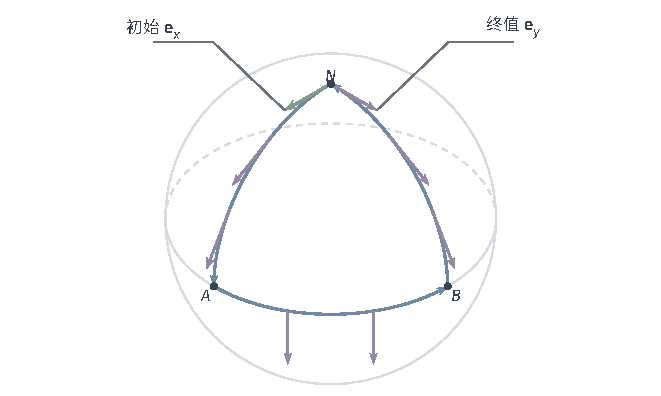
\includegraphics[width=112.0mm]{figures/00-shared/mathematical-preliminaries-upper/05-space-and-geometry/tikz/geometry-sphere-parallel-transport/figure.pdf}
  \caption{单位球面上沿$N\to A\to B\to N$的平行移动。
 蓝色为给定的三条大圆弧，紫箭头为例~\ref{ex:geometry-sphere-parallel-transport}
 中逐段计算的切向量。沿路协变导数为零，返回$N$后的方向却由初始箭头
 $\bm e_x$变为紫色终值箭头$\bm e_y$。
 箭头在三维中等长，投影到纸面后的长度可以不同。图为解析教学示例。}
 \label{fig:geometry-sphere-parallel-transport}
\end{figure}

这里的变换由路径和联络决定，不是任意选一个旋转来对齐环境向量。
前文群作用规定的是输入在指定变换下的响应；平行移动规定的是沿几何路径的方向比较，
即使二者有时都用矩阵表示，也不能据此互换。


球面闭路例子已经表明，搬运结果可以依赖路线。
为检测一个点附近的这种差异，可以比较沿两个方向先后求协变导数的结果。
方向场本身未必可交换，必须扣除$[\bm U,\bm V]$造成的变化，
剩下的才是联络对局部路径差异的响应。
这里有三个方向的不同职责：$\bm U,\bm V$指定小回路的两个方向，
另一个切向量$\bm W$是沿路搬运的箭头。给定前两个方向后，曲率作用在$\bm W$上，
检测绕路带来的方向变化；$\bm W$不必等于路径的前进速度。

\begin{definition}[Riemann曲率]
\label{def:geometry-riemann-curvature}
本章取曲率符号约定
\begin{equation}
 R(\bm U,\bm V)\bm W
 =\nabla_{\bm U}\nabla_{\bm V}\bm W
  -\nabla_{\bm V}\nabla_{\bm U}\bm W
  -\nabla_{[\bm U,\bm V]}\bm W.
 \label{eq:geometry-riemann-curvature}
\end{equation}
Levi--Civita联络的这个算子称为\term{Riemann曲率}（Riemann curvature）。
在点$\bm p$处，其值只依赖$\bm U,\bm V,\bm W$在该点的值，
而不依赖它们在附近的具体延拓。
\end{definition}
最后一项消掉方向场选择带来的导数项，使$R$成为按点定义的张量，即对点处方向多线性且不依赖坐标的对象。
例如在$\bm V$前乘光滑函数时，前两项会出现关于该函数的导数，
第三项恰好抵消它们。比较小闭路平行移动与恒等映射时，以闭路面积为尺度的
首项由$R(\bm u,\bm v)$控制；这个首项也可能为零，具体正负随绕行方向约定改变。
有限大闭路的总效应不能简单用某一点的曲率乘面积代替。

曲率算子仍含多个方向。选定一个二维切平面，可以用它给出一个标量曲率，
比较该平面内的局部几何。
\begin{definition}[截面曲率]
\label{def:geometry-sectional-curvature}
若$\bm u,\bm v\in T_{\bm p}\mathcal M$线性无关，
定义它们张成平面的\term{截面曲率}（sectional curvature）为
\begin{equation}
 K_{\bm p}(\bm u,\bm v)
 =\frac{g(R(\bm u,\bm v)\bm v,\bm u)}
 {g(\bm u,\bm u)g(\bm v,\bm v)-g(\bm u,\bm v)^2}.
 \label{eq:geometry-sectional-curvature}
\end{equation}
分母是该平行四边形的平方面积，正定性保证它为正。
\end{definition}
更换同一平面的基不改变比值。二维流形每点只有整个切平面这个选择，
所得量就是Gauss曲率；一维流形没有二维切平面，不能给圆硬套一个截面曲率数值。
一维Riemann曲率张量恒为零。

平面采用欧氏度量时，直角坐标中的联络系数为零，故$R=0$。
半径$R_0$的圆柱取局部参数
$(s,z)\mapsto(R_0\cos(s/R_0),R_0\sin(s/R_0),z)$，
诱导度量为$\mathrm ds^2+\mathrm dz^2$，
所以局部联络系数和内在曲率同样为零。
圆柱在环境中明显弯曲，却可以局部无伸缩地展开成平面；
把圆柱卷起来改变的是嵌入形状，不是这个局部度量。

为什么同样看上去是弯的，圆柱和球面却被分开？可以用一张纸做实验：
圆柱侧面可以由平整的纸不加拉伸、不打皱地卷成，纸上画的角度和距离在卷动后保持不变；
球面则做不到——把平纸贴到球面上，必然要在某些地方剪开或拉伸。
所以“弯”有两层含义：一层是从外面看形状是弯的（嵌入弯曲，圆、圆柱都有），
另一层是小块内部的距离规则与平面本质不同、无法摊平（内在曲率，只有球面这里非零）。
联络与曲率要检测的是后一层，这也是不能凭眼睛或坐标系数判断曲率的原因。

半径$R_0$的球面则不同。对切向场，微分
$\langle\bm V,\bm p\rangle=0$给出
$\langle\mathrm d\bm V(\bm U),\bm p\rangle=-\langle\bm V,\bm U\rangle$，
因此
\[
 \nabla_{\bm U}\bm V
 =\mathrm d\bm V(\bm U)+\frac{g(\bm U,\bm V)}{R_0^2}\bm p.
\]
将其代入曲率定义，环境二阶导数与交换子相消；
再投影时，法向系数的导数被消去，而$\mathrm d\bm p(\bm U)=\bm U$留下
\[
 R(\bm U,\bm V)\bm W
 =\frac1{R_0^2}\bigl(g(\bm V,\bm W)\bm U-g(\bm U,\bm W)\bm V\bigr).
\]
代入式~\eqref{eq:geometry-sectional-curvature}便得任意截面
$K=1/R_0^2>0$。这也核对了本章曲率符号：球面的曲率为正。

在图~\ref{fig:geometry-sphere-parallel-transport}所用的单位球面北极
$N=(0,0,1)^\top$，取正交单位切向量$\bm u=\bm e_x$、$\bm v=\bm e_y$。
若被搬运的箭头取$\bm W=\bm v$，上式具体给出
\[
 R(\bm u,\bm v)\bm v=\bm u,\qquad
 K_N(\bm u,\bm v)=
 \frac{g(\bm u,\bm u)}{1\cdot1-0^2}=1.
\]
分子读出曲率作用后沿$\bm u$的分量，分母消去所选两方向围成的面积平方的尺度。
这里计算的是北极附近一个截面的局部曲率；前面的三段球面图则展示有限闭路的最终搬运。
缩小回路后观察方向变化的首项，才把这种沿路变化与局部曲率联系起来。

第\ref{sec:geometry-sampled-local-linearization}节将估计切平面；其法向误差需要与内在曲率区分。圆的一维方向沿环境空间转动，
产生二阶法向偏离，但其内在Riemann曲率为零；
圆柱也有法向弯曲而内在平坦。二维开带本来就是平面的开集，
式~\eqref{eq:geometry-strip-metric}虽有随位置变化的系数，内在曲率仍为零。
这些例子说明，法向二阶误差和Christoffel系数都不能单独作为内在非零曲率的证据。
局部曲率也不替代拓扑：平面与圆柱局部同样平坦，整体的环却不同；
局部零曲率本身不保证任意全局闭路上的搬运都平凡。

\subsection{对象的位置更新}
\label{sec:geometry-position-updates}
\label{sec:geometry-geodesic-motion-minimization}

\label{sec:geometry-geodesic-motion}

给定当前位置和一个切向步，直接沿环境直线前进通常会离开流形。
让速度沿自身路径平行移动，在初值解存在的时间内，就能在保持初始速度大小的同时
产生流形内的新位置。对足够短的时间可以这样更新，全局延拓还需另外的条件。

以单位球面为例说明这个要求有多强。取$\bm p=(1,0,0)^\top$、切向量$\bm v=(0,1,0)^\top$，
则$\bm p+t\bm v=(1,t,0)^\top$的长度为$\sqrt{1+t^2}$，除$t=0$外都大于$1$，
所以沿环境直线走出的点全部落在球外。
若改为让$\bm v$沿路径自身保持长度和相对方向，轨迹就是大圆
$\gamma(t)=(\cos t,\sin t,0)^\top$，它始终在球面上。
注意$\gamma''(t)=-\gamma(t)$并不为零：环境加速度恒指向球心且垂直于球面，
是“贴住球面”所需要的，而不是球面内的转弯。
因此判定“沿球面直行”的标准不能是环境加速度为零，
而应是它的切向部分为零；下面的协变导数正是为此设计。

\begin{definition}[测地线]
\label{def:geometry-geodesic}
相对于Riemann流形的Levi--Civita联络，采用仿射参数的曲线$\gamma$若满足
\[
 \frac{D\dot\gamma}{\mathrm dt}=\bm0,
\]
称为\term{测地线}（geodesic）。
\end{definition}
它没有切向加速度，速度沿自身路径作平行移动。
度量相容进一步给出
$\frac{\mathrm d}{\mathrm dt}\lVert\dot\gamma\rVert_g^2
=2g(D\dot\gamma/\mathrm dt,\dot\gamma)=0$，因此速度大小恒定。
环境加速度仍可非零，例如球面大圆需要法向加速度才能留在球面。

“仿射参数”说明换元$t=ar+b$、$a\neq0$保留这个方程。
一般换元则产生
\[
 \frac{D}{\mathrm dr}\frac{\mathrm d\gamma}{\mathrm dr}
 =(\tau'(r))^2\frac{D\dot\gamma}{\mathrm dt}
   +\tau''(r)\dot\gamma.
\]
非匀速参数化可以描出相同几何轨迹，却不再满足零协变加速度。
因此不能把路径长度的任意重参数化不变性照搬到这个运动方程。

要在坐标中求解，先用式~\eqref{eq:geometry-koszul-formula}取
$\bm U=\partial_i,\bm V=\partial_j,\bm W=\partial_\ell$。
坐标方向交换子为零，于是
\[
 2\sum_k g_{k,\ell}\Gamma^k_{i,j}
 =\partial_i g_{j,\ell}+\partial_j g_{i,\ell}-\partial_\ell g_{i,j}.
\]
乘逆度量便得到Christoffel符号
\begin{equation}
 \Gamma^k_{i,j}
 =\frac12\sum_{\ell=1}^d g^{k,\ell}
  \left(\frac{\partial g_{\ell,j}}{\partial z^i}
       +\frac{\partial g_{i,\ell}}{\partial z^j}
       -\frac{\partial g_{i,j}}{\partial z^\ell}\right),
 \qquad [g^{i,j}]=\bm G^{-1}.
 \label{eq:geometry-christoffel-symbols}
\end{equation}
将$\bm V=\dot\gamma=\sum_j\dot z^j\partial_j$代入
式~\eqref{eq:geometry-covariant-derivative-along-path}，测地条件成为
\begin{equation}
 \ddot z^k+\sum_{i,j=1}^d
 \Gamma^k_{i,j}(\bm z)\dot z^i\dot z^j=0.
 \label{eq:geometry-geodesic-equation}
\end{equation}

测地方程描述的运动不依赖坐标，但这不意味着每个Christoffel系数都是几何不变量。
要辨明这些系数的含义，需要区分几何张量与一张普通分量表。
这里的几何张量（geometric tensor）是点处、与坐标无关的多线性对象；
换基只对它的各个输入和输出作线性变换。因此，零分量表换基后仍为零。
Christoffel符号不满足这一规律。例~\ref{ex:geometry-coordinate-connection}中，同一个正半轴的欧氏几何，
在$x$坐标中有$\Gamma^x_{x,x}=0$，改用$x=e^u$后却有$\Gamma^u_{u,u}=1$。
度量相应由$g_{x,x}=1$变成$g_{u,u}=e^{2u}$，代入
式~\eqref{eq:geometry-christoffel-symbols}也给出相同结果。
因此这些符号是联络的坐标系数，不是张量。
基向量的变化与这些系数共同组成协变加速度，后者及所得曲线仍是几何对象。

光滑系数使这个二阶方程在给定
$\gamma(0)=\bm p$、$\dot\gamma(0)=\bm v$后具有局部唯一解，
并光滑依赖初值。这里“局部”同时限制时间和坐标覆盖范围；
可以换图延拓，但若路径有限时间离开流形，延拓就会失败。
开单位球内的欧氏直线从原点出发，以速度$2\bm e_1$前进，
在$t=1/2$时便到达不属于该流形的边界，不能默认解存在至$t=1$。

\begin{definition}[指数映射]
\label{def:geometry-exponential-map}
对给定$\bm p$，若初速度$\bm v$的测地线$\gamma_{\bm v}$存在至$t=1$，
定义
\[
 \operatorname{Exp}_{\bm p}(\bm v)=\gamma_{\bm v}(1).
\]
它称为$\bm p$处的\term{指数映射}（exponential map），
其定义域至少包含$T_{\bm p}\mathcal M$中零向量的一个邻域。
\end{definition}
初速度缩放对应时间缩放：
$\operatorname{Exp}_{\bm p}(t\bm v)=\gamma_{\bm v}(t)$，只在两边均有定义时使用。
因而$\operatorname{Exp}_{\bm p}(\bm0)=\bm p$且
$\mathrm d(\operatorname{Exp}_{\bm p})_{\bm0}=\operatorname{id}_{T_{\bm p}\mathcal M}$。
逆函数定理保证在足够小邻域中它是微分同胚；
这为用切向量表示附近点提供了一种局部方式，不保证全局一一对应。

单位球面上，$\bm v\perp\bm p$、$r=\lVert\bm v\rVert_2$时，
\begin{equation}
 \operatorname{Exp}_{\bm p}(\bm v)
 =\cos r\,\bm p+\frac{\sin r}{r}\bm v,
 \label{eq:geometry-sphere-exponential}
\end{equation}
$r=0$时按连续延拓取$\bm p$。
对应曲线$\gamma(t)=\cos(tr)\bm p+\sin(tr)\bm v/r$
满足$\lVert\gamma(t)\rVert_2=1$、初速度为$\bm v$，
且$\ddot\gamma=-r^2\gamma$为纯法向，所以确实解测地线方程。
所有方向上长度为$\pi$的初速度都到达对跖点$-\bm p$；
即使映射处处有定义，也未必全局单射。

图~\ref{fig:vol1-add-geometry-exponential-noninjective}用单位圆截面展示同一终点的两种初速度。局部可逆性只保证足够小的切向量能够唯一记录附近点，不能用来把远处点与任意大切向步一一配对。
\begin{figure}[!htb]
  \centering
  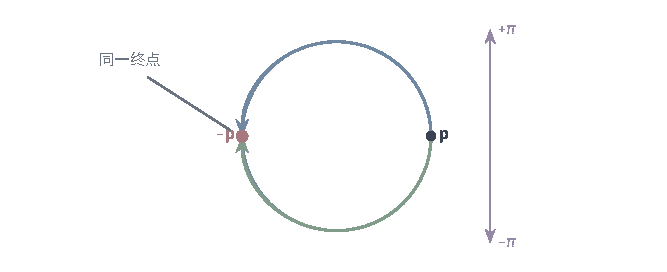
\includegraphics[width=112mm]{figures/00-shared/mathematical-preliminaries-upper/05-space-and-geometry/tikz/comprehension-additions/geometry-exponential-noninjective.pdf}
  \caption{指数映射的局部性。取单位圆上$\bm p=(1,0)^\top$，沿两个相反切方向分别走长度$\pi$，蓝、绿半圆都到达$-\bm p$。右侧$+\pi$与$-\pi$表示以单位切方向为基的初速度系数，图中箭头长度仅为示意。此例已足以说明指数映射可能不全局单射。}
  \label{fig:vol1-add-geometry-exponential-noninjective}
\end{figure}




切向量$\bm v$给出可行的瞬时方向，有限位移$\bm p+\bm v$却通常离开流形。
指数映射给出一种更新，但求解精确测地线可能昂贵。
如果只需保证一阶变化正确，可以使用更易计算的局部返回映射。

\begin{definition}[回缩]
\label{def:geometry-retraction}
对每个$\bm p$，在$T_{\bm p}\mathcal M$的零向量邻域中给定
$\mathcal R_{\bm p}(\bm v)\in\mathcal M$，并使其光滑依赖$(\bm p,\bm v)$。
若
\[
 \mathcal R_{\bm p}(\bm0)=\bm p,\qquad
 \mathrm d(\mathcal R_{\bm p})_{\bm0}[\bm v]=\bm v,
\]
则称这一族映射为\term{回缩}（retraction）。
\end{definition}
第一项保留起点，第二项保留初速度。它不要求沿$t\mapsto\mathcal R_{\bm p}(t\bm v)$
作精确测地运动，也不要求任意大步长都在定义域中。
指数映射是一种局部回缩，其他回缩可有不同的高阶误差。


这些映射接收当前位置与一个小切向步，输出新位置。
它们只规定一步怎样保持可行；怎样选择方向、步长以及整个序列是否收敛，是后面的求解与收敛问题。

\subsubsection{三维旋转的表示与更新}
\label{sec:geometry-so3-updates}

若未知对象是一个三维朝向，直接平均两张旋转矩阵通常破坏正交性。
要保持合法朝向，可以沿约束允许的切向更新，也可以改用带约束的四元数记录。
下面固定主动旋转列向量的约定：$\bm x'=\bm R\bm x$，
先作用$\bm R_1$、后作用$\bm R_2$的复合为$\bm R_2\bm R_1$
\scite{math-sola2017quaternion}。

\paragraph{正交约束与轴角更新}
保持长度和定向的三维矩阵组成\term{三维旋转群}（three-dimensional rotation group）
\[
 \mathrm{SO}(3)=\{\bm R\in\mathbb R^{3\times3}:\bm R^\top\bm R=\bm I,
 \ \det\bm R=1\}.
\]
乘法封闭、单位元是$\bm I$、逆是$\bm R^\top$，所以它确实是群。
对曲线$\bm R(t)$求导正交约束，得到
$\bm R^\top\dot{\bm R}+\dot{\bm R}^\top\bm R=\bm0$，故
\[
 T_{\bm R}\mathrm{SO}(3)=\{\bm R\bm\Omega:\bm\Omega^\top=-\bm\Omega\}.
\]
三阶斜对称矩阵由三个数决定，单位元处的空间记作$\mathfrak{so}(3)$。
反向的充分性由下面的指数路径给出：每个斜对称矩阵都能产生留在旋转群中的曲线。
用前面的叉积，把向量$\bm\omega=(\omega_1,\omega_2,\omega_3)^\top$写成
\[
 [\bm\omega]_\times=
 \begin{bmatrix}0&-\omega_3&\omega_2\\\omega_3&0&-\omega_1\\-\omega_2&\omega_1&0\end{bmatrix},
 \qquad [\bm\omega]_\times\bm x=\bm\omega\times\bm x.
\]
于是切向步$\bm R[\bm\omega]_\times$用三个数就能记录，
而不是任意改变九个矩阵元素。

对单位轴$\bm u$，叉积的分量展开给
$[\bm u]_\times^2=\bm u\bm u^\top-\bm I$、
$[\bm u]_\times^3=-[\bm u]_\times$。
方阵的指数由级数$\exp(\bm\Omega)=\sum_{j\geq0}\bm\Omega^j/j!$定义，由次乘性，各项范数不超过$\lVert\bm\Omega\rVert^j/j!$，级数对任意方阵绝对收敛。将其中的奇次项、偶次项分别汇总，得到\term{Rodrigues公式}
（Rodrigues' formula）
\begin{equation}
 \exp(\theta[\bm u]_\times)
 =\bm I+\sin\theta[\bm u]_\times+(1-\cos\theta)[\bm u]_\times^2.
 \label{eq:geometry-rodrigues}
\end{equation}
斜对称性保证指数与其转置相乘为$\bm I$；行列式沿连续曲线从$1$出发，
在正交矩阵的$\{-1,1\}$中只能保持$1$，所以该式始终产生合法旋转。
例如$\bm u=(0,0,1)^\top$、$\theta=\pi/2$时，
它把$(1,0,0)^\top$转到$(0,1,0)^\top$，并保持第三坐标不变。

反过来，每个三维旋转都可如此表示：实三阶正交矩阵在保定向条件下有特征值$1$，
取对应单位轴$\bm u$，其正交平面上的作用就是二维旋转。
这给出\term{轴角表示}（axis-angle representation）。
可以选$0\leq\theta\leq\pi$，其中$\cos\theta=(\operatorname{tr}\bm R-1)/2$；
恒等旋转的轴不唯一，$\theta=\pi$时相反轴也给同一旋转。
沿小角向量更新为$\bm R^+=\bm R\exp([\bm\omega]_\times)$，
它的一阶项是$\bm R+\bm R[\bm\omega]_\times$。
采用环境Frobenius诱导度量时，$\bm R\exp(t\bm\Omega)$还是测地线：
二阶导的左平移分量$\bm\Omega^2$对称，与所有斜对称切向分量正交，
所以环境加速度没有切向部分。矩阵群指数在这个指定度量下给出相应Riemann指数，
这不是任意流形或任意度量都具有的等同关系。

若改用三个依次绕坐标轴的角，记
$\bm R=\bm R_z(\alpha)\bm R_y(\beta)\bm R_x(\gamma)$，便得到一种欧拉角约定。
在$\beta=\pi/2$时，乘积化为
$\bm R_z(\alpha-\gamma)\bm R_y(\pi/2)$，只依赖两个角之差，
因此$\alpha,\gamma$不再能分别辨认；这就是\term{万向节锁}（gimbal lock）。
朝向本身仍合法，失效的是这组局部坐标，不能把坐标奇异误作物体失去了旋转自由度。

\paragraph{四元数记录与旋转复合}
另一种做法用四个数附加一个单位长度约束，从而避开上述欧拉角坐标的局部退化。
将\term{四元数}（quaternion）写成标量在前的二元组$q=(s,\bm u)$，
乘法规定为
\[
 (s,\bm u)(t,\bm v)
 =(st-\bm u^\top\bm v,\ s\bm v+t\bm u+\bm u\times\bm v).
\]
此处采用Hamilton乘法，乘积一般不可交换。
共轭$q^*=(s,-\bm u)$满足$qq^*=(s^2+\|\bm u\|_2^2,\bm0)$；
分量展开还能验证结合律及范数乘法性$\|pq\|_2=\|p\|_2\|q\|_2$。
单位四元数因而以$q^*$为逆。

把向量嵌入为纯虚四元数$(0,\bm x)$，用共轭作用定义
$q(0,\bm x)q^*=(0,\bm R(q)\bm x)$。
两次乘法展开给
\begin{equation}
 \bm R(q)\bm x
 =(s^2-\|\bm u\|_2^2)\bm x
 +2\bm u(\bm u^\top\bm x)+2s(\bm u\times\bm x),
 \qquad s^2+\|\bm u\|_2^2=1.
 \label{eq:geometry-quaternion-action}
\end{equation}
取$q=(\cos(\theta/2),\bm a\sin(\theta/2))$、$\|\bm a\|_2=1$，
上式就是绕$\bm a$的Rodrigues旋转。
因此半角来自两侧共轭作用，并非把物理角度减半。
例如$q=(\sqrt2/2,0,0,\sqrt2/2)$仍给绕第三轴$\pi/2$的旋转。

结合律使$\bm R(q_2q_1)=\bm R(q_2)\bm R(q_1)$，所以复合无需先转成矩阵。
$q$与$-q$却给出同一个作用；反过来，表示同一旋转的单位四元数也只差这个符号，
因为它们的商表示恒等旋转，而轴角式中这只给出$(1,\bm0)$或$(-1,\bm0)$。
这称为单位四元数对旋转群的\term{双覆盖}（double cover）。
四元数消除了欧拉角的这类坐标锁，却没有给每个旋转一个全局唯一的四维记录。
数值更新还须保持或重新归一化单位长度；非单位$q$的同一共轭式会附带缩放，不能直接称作旋转。

\paragraph{给定两次朝向的球面插值}
若要在两个朝向之间匀速转动，直接线性混合矩阵会破坏正交性，
直接线性混合单位四元数也通常不再保持单位长度。
先选两个单位代表$q_0,q_1$，当$q_0^\top q_1<0$时把$q_1$换成$-q_1$，
使$c=q_0^\top q_1\geq0$。这是利用双覆盖选择较短的旋转弧，而不是改变终点朝向。
令$\vartheta=\arccos c$，当$0<\vartheta\leq\pi/2$时定义
\begin{equation}
 q(t)=\frac{\sin((1-t)\vartheta)}{\sin\vartheta}q_0
       +\frac{\sin(t\vartheta)}{\sin\vartheta}q_1,
 \qquad 0\leq t\leq1.
 \label{eq:geometry-quaternion-slerp}
\end{equation}
这称为\term{球面线性插值}（spherical linear interpolation, SLERP）。
取$e=(q_1-cq_0)/\sin\vartheta$，则$q_0,e$正交且均为单位向量，
上式化为$q(t)=q_0\cos(t\vartheta)+e\sin(t\vartheta)$，
所以长度恒为$1$，在这张二维平面内沿大圆以恒定角速度前进。
物理旋转角是四元数球面角的两倍；符号选择使总转角不超过$\pi$。

例如从恒等朝向到绕第三轴$\pi/2$，中点四元数为
\[
 (\cos(\pi/8),0,0,\sin(\pi/8)),
\]
对应绕该轴$\pi/4$。
当$c=1$时用连续极限取常量$q(t)=q_0$；原始代表若互为对跖点，
它们表示同一朝向，先换符号即可使用这一情形。
若坚持插值指定的两个对跖四维向量，大圆不唯一，不能代入分母为零的式子。
当$c=0$时相对物理转角为$\pi$，两种终点符号都给同长度的最短旋转，
必须另作路径选择，不能宣称最短弧处处唯一。

\paragraph{旋转和平移的齐次复合}
朝向更新之外，刚体位姿还要移动原点。把$\bm x'=\bm R\bm x+\bm t$写为
\[
 \begin{bmatrix}\bm x'\\1\end{bmatrix}
 =\bm T\begin{bmatrix}\bm x\\1\end{bmatrix},
 \qquad
 \bm T=\begin{bmatrix}\bm R&\bm t\\\bm0^\top&1\end{bmatrix},
 \quad \bm R\in\mathrm{SO}(3).
\]
这些矩阵组成\term{三维刚体运动群}（three-dimensional rigid-motion group）$\mathrm{SE}(3)$。
分块乘法直接给出先$\bm T_1$后$\bm T_2$的结果
\[
 \bm T_2\bm T_1=
 \begin{bmatrix}\bm R_2\bm R_1&\bm R_2\bm t_1+\bm t_2\\\bm0^\top&1\end{bmatrix},
 \qquad
 \bm T^{-1}=\begin{bmatrix}\bm R^\top&-\bm R^\top\bm t\\\bm0^\top&1\end{bmatrix}.
\]
第一次的平移必须先换到第二次的方向下，不能只把$\bm t_1,\bm t_2$相加。
例如两次都绕第三轴转$\pi/2$，平移分别为$(1,0,0)^\top$和$(0,1,0)^\top$，
复合为绕该轴$\pi$并平移$(0,2,0)^\top$。
这里的齐次矩阵保持末坐标为$1$，属于前面射影变换的仿射特例；
它表示三维刚体作用，不含光学投影或透视除法。

\subsection{区域的体积计算}
\label{sec:geometry-riemannian-volume}

要比较区域的大小，路径的一维长度还不够，需要给小区域规定体积。
坐标切基围成的微小平行体，其平方体积是Gram行列式$\det\bm G$，
因此几何体积元为
\begin{equation}
 \mathrm dV_g=\sqrt{\det\bm G(\bm z)}\,\mathrm d\bm z.
 \label{eq:geometry-riemannian-volume}
\end{equation}
这是由度量产生的测度密度，不要求先为流形选定全局朝向。
一维时给出长度，二维时给出面积。
二维情形可以直接看出根号和行列式的来历：坐标切基$\partial_1,\partial_2$
张成的小平行四边形，其面积等于两向量构成的Gram矩阵行列式的平方根
（直角坐标时$\bm G=\bm I$，就退化为普通的$\mathrm dz^1\mathrm dz^2$）。
坐标网一旦被拉伸或歪斜，同一个参数小盒对应的真实面积就按这个比例放大或缩小，
所以不能再用$\mathrm d\bm z$本身当作面积。

图~\ref{fig:vol1-add-geometry-gram-volume}先用一个线性坐标网核对面积因子。单位参数方格经两条坐标方向张成平行四边形；边可以歪斜，真实面积仍由Gram行列式确定，而不是由两条边长直接相乘。
\begin{figure}[!htb]
  \centering
  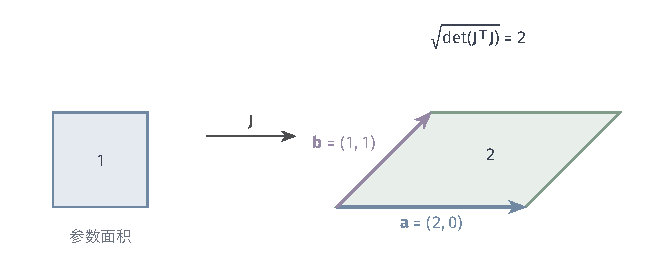
\includegraphics[width=112mm]{figures/00-shared/mathematical-preliminaries-upper/05-space-and-geometry/tikz/comprehension-additions/geometry-gram-volume.pdf}
  \caption{Gram行列式把参数面积换成真实面积。取$\bm J=\left[\begin{smallmatrix}2&1\\0&1\end{smallmatrix}\right]$，其列$\bm a=(2,0)^\top$、$\bm b=(1,1)^\top$围成面积为$2$的平行四边形。对应$\bm G=\bm J^\top \bm J$满足$\det \bm G=4$，故面积比例为$\sqrt{\det \bm G}=2$。左、右图使用相同长度比例，右侧面积恰为左侧的两倍。}
  \label{fig:vol1-add-geometry-gram-volume}
\end{figure}



坐标变换$\bm z=\psi(\bm v)$下，
$\det\widetilde{\bm G}=(\det\bm A)^2\det\bm G$，所以
\[
 \sqrt{\det\widetilde{\bm G}}\,\mathrm d\bm v
 =\sqrt{\det\bm G(\psi(\bm v))}\,|\det\bm A|\,\mathrm d\bm v.
\]
它正是多元积分换元中的Jacobian因子，故对可积函数所得积分不依赖坐标。
跨图时必须避免把重叠区域重复计数，可分割成可测片段分别积分；
光滑计算也可使用从属于图册、和为$1$的局部权重来拼接。

点带中$\sqrt{\det\bm G}=1+u/R>0$，
小盒$\mathrm ds\,\mathrm du$在外侧对应较大面积。
中心线限制为$u=0$后的一维体积元是$\mathrm ds$，不是把二维面积直接代入。
若样本相对几何体积有概率密度$q$，要求$q\geq0$且$\int q\,\mathrm dV_g=1$，
其分布测度才是$q\,\mathrm dV_g$；
当样本独立同分布地取自这个测度，且$\int|f|q\,\mathrm dV_g<\infty$时，
简单样本平均的期望是$\int fq\,\mathrm dV_g$；大数定律还保证它收敛到这个
加权积分。它并非自动近似$\int f\,\mathrm dV_g$。
几何体积与采样权重的差别将在离散平滑目标中再次出现。

当前开带无流形边界，但不是紧集。需要边界积分时，将另取有分片光滑边界的
截断闭域，并声明函数在边界的行为；不能只因图上画有虚线就把它当作同一个积分问题。

\Needspace{6\baselineskip}
\section{方程与优化}
\label{sec:geometry-equations-optimization}

前面的运算可以计算已知点或方向的响应，现在用它们求未知对象。
给定两两距离时，未知量是一组坐标；给定位置与速度时，未知量是一条运动轨迹。
若改为给定两个端点，还需比较允许路线的长度。最后在流形中寻找目标值最小的点，
其可行更新将调用微分、度量和回缩。

\subsection{距离信息下的坐标重构}
\label{sec:geometry-distance-coordinate-embedding}

设点数$n$为正整数，且只知道这些点之间的距离，能否给它们安排欧氏坐标，并精确保留这些距离？
这类问题在实际中很自然：测量设备往往只能给出物体上若干标记点两两之间的距离，
却没有一个共同的外部坐标系。要回答“能否重建”，先得看清距离丢掉了什么：
把整组点一起平移，所有距离都不变。也就是说，距离本身不携带原点信息，
所以恢复坐标前必须先人为固定一个位置基准（下面取点云重心为原点）；
后面还会看到，旋转和反射同样无法由距离辨认。
先从反方向计算。将$\bm y_1,\ldots,\bm y_n\in\mathbb R^d$按行组成
$\bm Y\in\mathbb R^{n\times d}$。\BookDefinitionRef{def:linear-algebra-gram-matrix}{定义~\ref{def:linear-algebra-gram-matrix}}中的
Gram矩阵$\bm B=\bm Y\bm Y^\top$记录两两内积，平方距离则为
\begin{equation}
  \delta_{i,j}=\lVert\bm y_i-\bm y_j\rVert_2^2
  =b_{i,i}+b_{j,j}-2b_{i,j}.
  \label{eq:geometry-distance-from-gram}
\end{equation}
距离不记录原点：将全部点平移同一个向量，差向量不变，内积却会改变。
因此从距离恢复内积前，需要先固定平移自由度。

把点云均值选为原点。令$\bm1\in\mathbb R^n$为全一向量，定义
\begin{equation}
  \bm J=\bm I_n-\frac1n\bm1\bm1^\top.
  \label{eq:geometry-centering-matrix}
\end{equation}
它满足$\bm J^\top=\bm J$、$\bm J^2=\bm J$和$\bm J\bm1=\bm0$；
$\bm J\bm Y$从每行减去样本均值。若$\bm\Delta=[\delta_{i,j}]$，
式~\eqref{eq:geometry-distance-from-gram}写成
\[
  \bm\Delta=\operatorname{diag}(\bm B)\bm1^\top
  +\bm1\operatorname{diag}(\bm B)^\top-2\bm B.
\]
左右各乘$\bm J$，前两项消失。对于已中心化的坐标，
$\bm J\bm Y=\bm Y$，于是
\begin{equation}
  \bm B=-\frac12\bm J\bm\Delta\bm J.
  \label{eq:geometry-double-centering}
\end{equation}
这称为\term{双重中心化}（double centering）：在两个点索引上消去均值项，
把平方距离转成以点云中心为原点的内积。此时尚未作低维投影。

任何真实坐标产生的Gram矩阵都半正定，因为
$\bm c^\top\bm B\bm c=\lVert\bm Y^\top\bm c\rVert_2^2\geq0$。
要证明这个条件也足够，需要排除双重中心化过程中丢失了某种非零距离差。

\begin{lemma}[双重中心化核的形式]
\label{lem:geometry-double-centering-kernel}
若对称矩阵$\bm H\in\mathbb R^{n\times n}$满足$\bm J\bm H\bm J=\bm0$，
则存在$\bm a\in\mathbb R^n$使
$\bm H=\bm1\bm a^\top+\bm a\bm1^\top$。
若另有$h_{i,i}=0$对全部$i$成立，则$\bm H=\bm0$。
\end{lemma}
\begin{proof}
令$\bm m=\bm H\bm1/n$、$\mu=\bm1^\top\bm H\bm1/n^2$。展开假设得到
\[
  \bm H=\bm1\bm m^\top+\bm m\bm1^\top-\mu\bm1\bm1^\top.
\]
取$\bm a=\bm m-(\mu/2)\bm1$即得所需形式。其对角元为$h_{i,i}=2a_i$，
故零对角条件迫使每个$a_i=0$，进而$\bm H=\bm0$。
\end{proof}

\begin{theorem}[有限距离的欧氏坐标重构]
\label{thm:geometry-euclidean-distance-embedding}
设$\bm\Delta\in\mathbb R^{n\times n}$对称且对角元为零，并令
$\bm B=-\bm J\bm\Delta\bm J/2$。矩阵$\bm\Delta$是某组欧氏点的平方距离矩阵，
当且仅当$\bm B$半正定。精确保留全部距离所需的最小欧氏维数为
$r=\operatorname{rank}(\bm B)$。
\end{theorem}
\begin{proof}
若已有欧氏点，先中心化，式~\eqref{eq:geometry-double-centering}便给出
$\bm B=\bm Y\bm Y^\top$，所以$\bm B$半正定。

反过来，半正定性和谱定理给出紧谱分解
$\bm B=\bm Q_r\bm\Lambda_r\bm Q_r^\top$，其中$\bm\Lambda_r$含$r$个正特征值。
取
\begin{equation}
  \bm Y=\bm Q_r\bm\Lambda_r^{1/2},
  \label{eq:geometry-classical-scaling-coordinates}
\end{equation}
则$\bm Y\bm Y^\top=\bm B$。又因$\bm B\bm1=\bm0$，
$\lVert\bm Y^\top\bm1\rVert_2^2=\bm1^\top\bm B\bm1=0$，坐标已中心化。
用式~\eqref{eq:geometry-distance-from-gram}从$\bm B$生成$\bm\Delta'$。
$\bm\Delta'$与$\bm\Delta$的双重中心化均为$\bm B$，两者之差对称、
对角为零且双重中心化为零。前一引理遂给出$\bm\Delta'=\bm\Delta$。

任意$\mathbb R^k$中的坐标矩阵所产生的Gram矩阵秩至多为$k$，
因此精确重构要求$k\geq r$；上述构造又在$k=r$时达到要求。
$r=0$时全部点重合，可视为嵌入零维空间。
\end{proof}

这个判据是经典尺度分析的代数核心。$\bm B$有负特征值时，输入关系不能被精确实现为
欧氏平方距离。逐对测量的距离误差可能造成负谱；直接由一组带噪坐标精确计算的距离
却仍来自欧氏点，其Gram矩阵不会仅因坐标带噪而失去半正定性。后者重构的是观测点，
不是噪声发生前的潜在点。

距离保留了相对位置，却不能确定绝对位置、朝向或手性。对正交矩阵
$\bm Q\in\mathbb R^{r\times r}$和平移$\bm a$，令
$\widetilde{\bm y}_i=\bm Q\bm y_i+\bm a$，则
\[
 \lVert\widetilde{\bm y}_i-\widetilde{\bm y}_j\rVert_2
 =\lVert\bm Q(\bm y_i-\bm y_j)\rVert_2
 =\lVert\bm y_i-\bm y_j\rVert_2.
\]
正交变换既含旋转，也含反射。中心化只消去平移，不能选择唯一朝向。

对于中心化的最小维坐标，这也是全部不确定性。设
$\bm Y,\widetilde{\bm Y}\in\mathbb R^{n\times r}$均列满秩并产生相同距离，
则双重中心化给出相同$\bm B$。它们的列空间都等于$\bm B$的值域。
对$\bm B=\bm Q_r\bm\Lambda_r\bm Q_r^\top$定义
$\bm M=\bm\Lambda_r^{-1/2}\bm Q_r^\top\bm Y$，可得
\[
 \bm Y=\bm Q_r\bm\Lambda_r^{1/2}\bm M,\qquad
 \bm M\bm M^\top
 =\bm\Lambda_r^{-1/2}\bm Q_r^\top\bm B\bm Q_r
   \bm\Lambda_r^{-1/2}=\bm I_r.
\]
方阵$\bm M$因而正交。写$\bm M=\bm U^\top$，对另一组坐标同样得到
$\widetilde{\bm Y}=\bm Q_r\bm\Lambda_r^{1/2}\widetilde{\bm U}^\top$，
于是$\widetilde{\bm Y}=\bm Y\bm U\widetilde{\bm U}^\top$。
重复特征值允许坐标轴在对应子空间内旋转；更高维实现的额外方向不含点云信息，
两组点仍在各自张成空间之间具有保距正交对应。

\begin{example}[三个点能否放在一条直线上]
\label{ex:geometry-three-point-embedding}
取$\bm y_1=(-1,0)^\top$、$\bm y_2=(0,1)^\top$、
$\bm y_3=(1,0)^\top$，其均值是$(0,1/3)^\top$。平方距离与中心化结果为
\[
 \bm\Delta=\begin{bmatrix}0&2&4\\2&0&2\\4&2&0\end{bmatrix},
\]
\begin{equation}
 -\frac12\bm J\bm\Delta\bm J
 =\begin{bmatrix}
  10/9&-2/9&-8/9\\
  -2/9&4/9&-2/9\\
  -8/9&-2/9&10/9
 \end{bmatrix}.
 \label{eq:geometry-three-point-centered-gram}
\end{equation}
正特征值为$2$和$2/3$，所以精确重构需要二维。
若只保留特征值$2$对应的水平方向，端点间距离仍为$2$，
顶点到两端的距离却从$\sqrt2$变成$1$；这是一种近似，不是另一份精确坐标。
\end{example}

这里必须区分谱近似的目标。若$\bm B$半正定，保留最大$k<r$个特征值时，
\BookTheoremRef{thm:matrix-analysis-best-low-rank}{定理~\ref{thm:matrix-analysis-best-low-rank}}保证Gram矩阵的Frobenius误差最小，
平方误差为$\sum_{j>k}\lambda_j^2$。在一组给定中心化坐标上作对应PCA投影，
坐标平方重构误差则为$\sum_{j>k}\lambda_j$。若原距离为
$d_{i,j}=\sqrt{\delta_{i,j}}$，近似坐标为$\widetilde{\bm y}_i$，
还可以直接比较逐对距离，例如把距离应力（distance stress）取为
\[
 \sum_{i<j}
 \bigl(\lVert\widetilde{\bm y}_i-\widetilde{\bm y}_j\rVert_2-d_{i,j}\bigr)^2.
\]
它比较距离，前两种误差分别比较内积和坐标，因此优化目标不同。
最大相对距离误差则比较
\[
 \max_{\substack{i<j\\d_{i,j}>0}}
 \frac{\bigl|\lVert\widetilde{\bm y}_i-\widetilde{\bm y}_j\rVert_2-d_{i,j}\bigr|}
 {d_{i,j}}.
\]
全体点重合时不使用这个比值准则。对含负谱的$\bm B$，保留最大的至多$k$个正特征值给出
半正定秩至多$k$约束下的Frobenius近似；舍弃负谱的大小仍须与测量误差比较。

例~\ref{ex:geometry-three-point-embedding}中的三个点都落在单位圆上，
但精确保留弦长需要二维欧氏坐标；这个维数描述有限距离矩阵的重构要求。
圆本身在每个点附近只需一个角度坐标，内在维数仍为一。
因此有限点的最小欧氏重构维数与潜在连续模型的局部自由度是不同对象，
不能把保弦长的二维结果直接当作潜在流形二维的证据。
要判断连续模型，还需结合局部方向、沿模型的距离以及邻域粘合关系。

\subsection{初值条件下的测地轨迹求解}
\label{sec:geometry-geodesic-initial-value}

给定$\gamma(0)=\bm p$与$\dot\gamma(0)=\bm v$，求满足
式~\eqref{eq:geometry-geodesic-equation}的轨迹。把二阶方程改写为$(z,\dot z)$的一阶系统，
局部光滑系数保证解在初值附近存在唯一。这里固定的是位置与速度，不是两个端点。
在重叠坐标图中，已有解与换图后的解由唯一性拼接，从而得到最大延拓区间。
只要位置与速度留在一组系数受控的紧区域内，就可继续局部求解；
流形缺口或无界离开会阻止这个过程。

完整单位球面上，取$\bm p\in\mathbb S^{D-1}$、$\bm v\perp\bm p$，则
$\gamma(t)=\cos(t\lVert\bm v\rVert_2)\bm p
+\sin(t\lVert\bm v\rVert_2)\bm v/\lVert\bm v\rVert_2$
对全部$t$存在，$\bm v=\bm0$时取恒定轨迹。开球的直线却可能有限时间到达缺失边界。
第\ref{sec:geometry-endpoint-minimizing-path}节的完备性条件将给出全局延拓保证，
但初值的唯一性并不保证指定端点之间只有一条路径。

\subsection{端点约束下的最短路径求解}
\label{sec:geometry-endpoint-minimizing-path}

现在给定$\bm p,\bm q$，要求找到达到
式~\eqref{eq:geometry-geodesic-distance}下确界的路径。
直接把长度积分拿来做变分并不方便：根号里含速度，求导后形式复杂。
一个常用替代是在固定时间区间上改用“动能型”的能量积分；
下面将看到，走得忽快忽慢只会白白增加能量，因此能量最小的路径必然匀速，
而匀速时能量与长度的平方成正比，二者的最优路径一致。其与测地方程的联系可通过路径能量建立。固定时间区间$[a,b]$，定义
\[
 E(\gamma)=\frac12\int_a^b\lVert\dot\gamma\rVert_g^2\,\mathrm dt.
\]
由Cauchy--Schwarz不等式，
$L_g(\gamma)^2\leq2(b-a)E(\gamma)$，等号恰对应几乎处处恒定的速度大小。
因此对可作匀速参数化的非退化路径，最小化长度可联系到固定时间的能量最小化；
能量本身却不具有长度那样的任意重参数化不变性。

在局部坐标中，Lagrange函数为
$\mathscr L(\bm z,\dot{\bm z})=\frac12\sum_{i,j}g_{i,j}(\bm z)\dot z^i\dot z^j$。
取光滑扰动$\bm h$，满足$\bm h(a)=\bm h(b)=\bm0$，并令
$\bm z_\varepsilon(t)=\bm z(t)+\varepsilon\bm h(t)$。
取足够小的$\varepsilon$使路径仍在坐标域内。
若$\varphi$为当前坐标的参数化，一阶变分就是把整条路径沿这个方向改变后，
能量关于扰动幅度的导数：
\[
 \delta E[\bm h]
 =\left.\frac{\mathrm d}{\mathrm d\varepsilon}
 E(\varphi\circ\bm z_\varepsilon)\right|_{\varepsilon=0}.
\]
对积分求导并分部积分，得到
\[
 \delta E[\bm h]
 =\int_a^b\sum_k\left(
 \frac{\partial\mathscr L}{\partial z^k}
 -\frac{\mathrm d}{\mathrm dt}
     \frac{\partial\mathscr L}{\partial\dot z^k}\right)h^k\,\mathrm dt.
\]
边界项因固定端点消失。驻定要求任意这样的$\bm h$都使变分为零，
因此括号中每个系数都必须为零：若某个连续系数在一点非零，
就在它保持同号的小邻域内取一个同号、光滑且在邻域外为零的扰动，
相应积分便不为零，产生矛盾。计算括号中的两个偏导得
\[
 \begin{aligned}
 \frac{\partial\mathscr L}{\partial z^k}
   &=\frac12\sum_{i,j}\partial_k g_{i,j}\dot z^i\dot z^j,\\
 \frac{\mathrm d}{\mathrm dt}
    \frac{\partial\mathscr L}{\partial\dot z^k}
   &=\sum_j g_{k,j}\ddot z^j+
     \sum_{i,j}\partial_i g_{k,j}\dot z^i\dot z^j.
 \end{aligned}
\]
对第二行的速度乘积对称化后，Euler--Lagrange方程为
\[
 \sum_jg_{k,j}\ddot z^j+
 \frac12\sum_{i,j}
  (\partial_i g_{k,j}+\partial_j g_{k,i}-\partial_k g_{i,j})
  \dot z^i\dot z^j=0.
\]
乘$\bm G^{-1}$即得式~\eqref{eq:geometry-geodesic-equation}。
跨图路径可对各段内支撑的扰动分别推导，得到相同几何方程。
这说明光滑匀速最短路必为测地线，不说明每个能量驻点都是最短路。

指数映射给出描述这些局部路径的区域。取零切向量附近的小开集$V$，
要求$\bm v\in V$时$t\bm v\in V$对$0\leq t\leq1$成立，
且$\operatorname{Exp}_{\bm p}$在$V$上为微分同胚。
它的像称为$\bm p$的正规邻域（normal neighborhood），
其中每个点都用一个初速度表示，径向路径对应$t\bm v$。
长度比较还需要指数映射的另一性质：Gauss引理说明，径向单位速度与
固定半径的横向变化正交，且径向速度的长度保持不变。这里引用该引理，
用它说明最短性怎样得出。把$V$缩成切空间中的小球，记竞争路径为
$\gamma(t)=\operatorname{Exp}_{\bm p}(r(t)\bm u(t))$，其中$\lVert\bm u(t)\rVert_g=1$。
在$r(t)>0$的部分，径向与横向速度正交，故
\[
 \lVert\dot\gamma(t)\rVert_g^2
 =\dot r(t)^2+
 \bigl\lVert\mathrm d(\operatorname{Exp}_{\bm p})_{r(t)\bm u(t)}
              [r(t)\dot{\bm u}(t)]\bigr\rVert_g^2
 \geq\dot r(t)^2.
\]
因此，从中心$\bm p$到$\bm q=\operatorname{Exp}_{\bm p}(\bm v)$、
始终留在此邻域内的任意路径，长度至少为
$\int|\dot r(t)|\,\mathrm dt\geq\lVert\bm v\rVert_g$。
经过中心时可分段取极限，结论不变。
径向路径$t\mapsto\operatorname{Exp}_{\bm p}(t\bm v)$恰有这个长度，因而在邻域内最短。
还可进一步选择凸正规邻域（convex normal neighborhood），
让其中任意两点由唯一的邻域内最短测地线连接，整条线段留在该邻域中。
这里“凸”指测地线连接的性质，不是要求环境中的欧氏直线段留在区域内。
凸正规邻域的存在性在这里作为进一步的局部结论引用；上述径向比较说明了
长度最短性所需的额外依据，不能只凭微分方程的存在唯一性得到。
离开这种局部范围后，其他路线可能更短。
若一段测地线达到$d_g$，称为\term{长度最短测地线}（length-minimizing geodesic）。

完整单位圆上，从$(1,0)^\top$到$(0,-1)^\top$的逆时针弧长为$3\pi/2$，
顺时针弧长为$\pi/2$。两条匀速圆弧都满足零协变加速度，
只有后者达到距离。这两条路线的初速度方向不同；局部初值解的唯一性不能代替全局路线的长度比较。
测地线规定局部怎样运动，距离比较全部允许路线的长度下确界，最短路则要求某条路线真正达到它。
圆上长弧与短弧说明第一项不推出第三项；前面的穿孔平面又说明下确界存在也不保证达到。
更精细的失去最短性判据不在本章展开；下面先回答哪些条件能保证最短路存在。

\begin{theorem}[Hopf--Rinow定理的最短路存在性结论]
\label{thm:geometry-hopf-rinow-existence}
设$(\mathcal M,g)$为有限维、连通、无边界的光滑Riemann流形。
若它关于$d_g$完备，则任意两点之间存在长度最短测地线。
此时任意初速度的测地运动也可以延拓到所有实数时间。
\end{theorem}
这里引用这一定理的存在性结论，不展开完整等价条件及证明。
完备性是每个$d_g$-Cauchy序列都在$\mathcal M$内收敛；
它限制了路径是否能在有限长度内跑到空间缺口。
结论保证存在而不保证唯一：球面的对跖点之间有多条最短大圆弧，
指数映射仍不是全局单射。紧致无边界的Riemann流形满足这里的完备性条件。

穿孔平面给出省略完备性的反例。用欧氏诱导度量连接
$(-1,0)^\top$和$(1,0)^\top$，
沿横轴走到$(-\varepsilon,0)^\top$，绕半径$\varepsilon$的半圆，
再沿横轴到终点，长度为
\[
 (1-\varepsilon)+\pi\varepsilon+(1-\varepsilon)
 =2+(\pi-2)\varepsilon\longrightarrow2.
\]
环境距离给出下界$2$，所以$d_g=2$。
长度等于端点欧氏距离的路径只能沿连接线段前进，该线段经过被删去的原点，
故没有允许路径达到下确界。这里仍有局部测地解，却没有这两个端点的最短路。

\subsection{流形约束下的点优化}
\label{sec:geometry-point-optimization}
\label{sec:geometry-manifold-optimization}
\label{sec:geometry-point-optimality}

考虑$\min_{\bm p\in\mathcal M}f(\bm p)$，其中$f$为至少二阶连续可微的实函数。
流形约束已经包含在可行域中。普通偏导给出坐标变化，
但实际可行的一阶变化属于$T_{\bm p}\mathcal M$；
有限步更新还必须从切空间返回流形。

为什么不能直接沿用\BookChapterRef{chap:optimization}{第\ref{chap:optimization}章}的无约束下降法？
在平面上，更新$\bm p-\alpha\nabla f(\bm p)$只需要一次减法；
在球面上，同一个式子一般给出球外的点。
若改用坐标偏导$\nabla_{\bm z}f$作为方向，选不同的坐标图会得到不同的更新方向，
因为偏导数值依赖坐标刻度，而“最陡”是一个几何判断。
这正是需要梯度的原因：先由$f$确定一个与坐标无关的线性读取$\mathrm df_{\bm p}$，
再用度量把它转换成切向量，得到$\operatorname{grad}f$，
最后用回缩把切向步落到球面上。
以球面上的$f(\bm p)=-\bm a^\top\bm p$为例，环境梯度是常数$-\bm a$，
在$\bm p$处的可行下降方向却必须剔除法向分量，得到
$-\operatorname{grad}f=\bm a-(\bm a^\top\bm p)\bm p$。
目标本身并不复杂，困难全部来自可行域的弯曲。


在选择迭代方法以前，先检查这个最小值是否存在。若非空流形$\mathcal M$紧致且$f$连续，
极小值定理保证全局最小值存在；非紧空间上可用紧的非空下水平集等条件替代，
不能只凭可微性保证存在。局部极小只和附近可行点比较，全局极小则和全部可行点比较。
以下最优性条件讨论无边界流形的点，不覆盖另加不等式所造成的活动边界。

第\ref{sec:geometry-tangent-maps}节已将微分$\mathrm df_{\bm p}$定义为对切向量的线性读取。
要从这个读取规则选出最陡方向，还需用度量把它表示成向量。
\begin{definition}[Riemann梯度]
\label{def:geometry-riemannian-gradient}
给定光滑函数$f$，点$\bm p$处的\term{Riemann梯度}（Riemannian gradient）
是由下式唯一确定的切向量$\operatorname{grad}f(\bm p)$：
\begin{equation}
 g_{\bm p}(\operatorname{grad}f,\bm v)=\mathrm df_{\bm p}(\bm v)
 \qquad(\bm v\in T_{\bm p}\mathcal M)
 \label{eq:geometry-riemannian-gradient-definition}
\end{equation}
\end{definition}
有限维内积的正定性保证存在唯一的表示向量。
微分由$f$决定，梯度还依赖度量；改变度量会改变最陡方向，但不改变微分是否为零。
在非驻点处，由Cauchy--Schwarz不等式，在$\lVert\bm v\rVert_g=1$的方向中，
$\mathrm df(\bm v)$最小为$-\lVert\operatorname{grad}f\rVert_g$，
并在负梯度的单位方向达到。驻点处各切向方向的一阶变化都为零。

设$\widehat f=f\circ\varphi$为坐标表达，为简洁把其偏导列表写作
\[
 \nabla_{\bm z}f=(\partial_1\widehat f,\ldots,\partial_d\widehat f)^\top.
\]
若梯度坐标为$\bm a$，则对所有坐标向量$\bm v$有
$\bm a^\top\bm G\bm v=\nabla_{\bm z}f^\top\bm v$，所以
\begin{equation}
 [\operatorname{grad}f]_{\bm z}=\bm G^{-1}\nabla_{\bm z}f.
 \label{eq:geometry-riemannian-gradient-coordinates}
\end{equation}
偏导列表表示余切向量，逆度量把它转为切向量；只有特定正交归一坐标中二者分量相同。
这里可以看清“偏导数为什么不等于梯度”。偏导数回答的是
“沿第$i$条坐标线移动时$f$变化多快”，它是一组读取规则；
而“最陡下降方向”需要先规定怎样量长度（度量），再在单位长度的方向中比谁使$f$下降最快。
坐标网可以任意拉伸：换一套坐标，各条坐标线上“走一格”的真实长度变了，
偏导数值跟着变，但同一条最陡下降线在曲面上的位置不应变。
乘上$\bm G^{-1}$正是把随刻度变化的读数，换算成与坐标无关的方向向量。
对欧氏诱导度量，若$f$有环境光滑延拓$\bar f$，则
$\operatorname{grad}f(\bm p)=\bm P_{\bm p}\nabla\bar f(\bm p)$，
因为投影不改变与任一切向量的内积。

梯度的一阶变化属于不同位置的切空间，不能直接求差后当作二阶信息。
联络给出所需的比较规则。此前联络接受的是向量场，现在要在单点沿给定速度求导。
对$\bm v\in T_{\bm p}\mathcal M$，任选局部光滑场$\bm V$满足$\bm V(\bm p)=\bm v$，
把$(\nabla_{\bm V}\operatorname{grad}f)(\bm p)$简记为$\nabla_{\bm v}\operatorname{grad}f$。
这与延拓无关：两种延拓之差在局部基中的系数都在$\bm p$处为零，
联络对第一个变量按光滑函数线性，故它们给出的导数在该点相同。
\begin{definition}[Riemann Hessian]
\label{def:geometry-riemannian-hessian}
在Levi--Civita联络下，定义\term{Riemann Hessian}（Riemannian Hessian）为线性算子
\[
 \operatorname{Hess}f(\bm p)[\bm v]
 =\nabla_{\bm v}\operatorname{grad}f
 \quad\text{从 }T_{\bm p}\mathcal M\text{ 到自身}.
\]
其双线性形式为
$\operatorname{Hess}f(\bm u,\bm v)
=g(\bm u,\operatorname{Hess}f[\bm v])$。
\end{definition}
度量相容和无挠使双线性形式对称。具体地，
\[
 g(\nabla_{\bm U}\operatorname{grad}f,\bm V)
 =\bm U(\bm V f)-(\nabla_{\bm U}\bm V)f;
\]
交换$\bm U,\bm V$后的差为
$[\bm U,\bm V]f-(\nabla_{\bm U}\bm V-\nabla_{\bm V}\bm U)f=0$。
在坐标中双线性形式的矩阵是
\begin{equation}
 B_{i,j}=\partial_i\partial_j\widehat f
             -\sum_k\Gamma^k_{i,j}\partial_k\widehat f,
 \qquad [\operatorname{Hess}f]_{\bm z}=\bm G^{-1}\bm B.
 \label{eq:geometry-hessian-coordinates}
\end{equation}
矩阵$\bm B$对称；线性算子的坐标矩阵$\bm G^{-1}\bm B$一般不是普通转置意义的
对称矩阵，却相对于内积$\bm G$自伴。非驻点处不能省略联络修正项。

沿任意$C^2$曲线，对$f(\gamma(t))$再求一次导数可得
\begin{equation}
 \frac{\mathrm d^2}{\mathrm dt^2}f(\gamma(t))
 =g(\operatorname{Hess}f[\dot\gamma],\dot\gamma)
   +g(\operatorname{grad}f,D\dot\gamma/\mathrm dt).
 \label{eq:geometry-function-second-derivative}
\end{equation}
测地线上第二项为零。因此，在无边界的局部极小点$\bm p_*$，
任意初速度的测地线都给出一元局部极小，必要条件为
\[
 \operatorname{grad}f(\bm p_*)=\bm0,\qquad
 g(\operatorname{Hess}f(\bm p_*)[\bm v],\bm v)\geq0
 \quad\text{对所有 }\bm v.
\]
若梯度为零且Hessian正定，指数坐标中的二阶Taylor展开给出严格局部极小。
半正定只给必要性，仍需更高阶信息；梯度为零也可能是极大点或鞍点。

欧氏凸性不能不加条件地移到弯曲可行域，因为连接两点的环境线段未必可行。
一种替代条件是\term{测地凸性}（geodesic convexity）：
在一个任意两点都可由域内最短测地线连接的区域$\Omega$上，
若$f$沿每条这样的仿射参数测地线都是一元凸函数，就称其在该区域测地凸。
此时对从$\bm p$到$\bm q$的此类路径，一元凸性给出
$f(\bm q)\geq f(\bm p)+\mathrm df_{\bm p}(\dot\gamma(0))$
（参数区间取$[0,1]$）；故域内驻点是域内全局极小。
区域是否具有所需连接性质、函数是否满足沿路凸性，都须验证，
不能由“目标来自欧氏凸函数”自动推出。

\subsubsection{基于梯度与回缩的一阶求解}
\label{sec:geometry-riemannian-gradient-method}

用括号上标记录迭代步，梯度更新写成
\begin{equation}
 \bm p^{(k+1)}=\mathcal R_{\bm p^{(k)}}
       (-\alpha^{(k)}\operatorname{grad}f(\bm p^{(k)})).
 \label{eq:geometry-riemannian-gradient-step}
\end{equation}
回缩的一阶相容性保证，沿该搜索曲线在$\alpha=0$处
\[
 \frac{\mathrm d}{\mathrm d\alpha}
 f(\mathcal R_{\bm p}(-\alpha\operatorname{grad}f))
 \bigg|_{\alpha=0}=-\lVert\operatorname{grad}f\rVert_g^2.
\]
因此非驻点处足够小的正步长确实下降。可以在回缩定义域内回溯，检验
$f(\bm p^{(k+1)})\leq f(\bm p^{(k)})
-c\alpha^{(k)}\lVert\operatorname{grad}f(\bm p^{(k)})\rVert_g^2$，
其中$0<c<1$。这只是逐步下降机制；
若还要推出梯度范数趋零，通常需紧的下水平集、目标下界、
回缩拉回函数的统一局部光滑界和相应回溯规则。
非凸问题不能因此保证全局极小，梯度范数趋零也不等于迭代点必然收敛。

\begin{example}[球面上的归一化更新]
\label{ex:geometry-sphere-retraction}
单位球面上$\bm p^\top\bm v=0$，故
$\lVert\bm p+\bm v\rVert_2=\sqrt{1+\lVert\bm v\rVert_2^2}$。取
\begin{equation}
 \mathcal R_{\bm p}(\bm v)
 =\frac{\bm p+\bm v}{\sqrt{1+\lVert\bm v\rVert_2^2}}.
 \label{eq:geometry-sphere-retraction}
\end{equation}
结果始终在球面上，零点导数为$\bm v$，所以是回缩。
设$r=\lVert\bm v\rVert_2>0$，回缩终点与起点的夹角为$\arctan r$。
指数映射则沿同一大圆行进长度$r$；当$0<r<\pi$时，这也等于两个端点的夹角。
二者只在小步长下接近，不是同一更新。

例如$f(\bm p)=-\bm a^\top\bm p$、$\bm a\neq\bm0$，
有$\operatorname{grad}f=-\bm a+(\bm a^\top\bm p)\bm p$。
先将环境下降方向$\bm a$投影到当前切空间，得到$-\operatorname{grad}f$，
再由归一化回缩把切向步变成球面上的新点。
驻点为$\pm\bm a/\lVert\bm a\rVert_2$；
在切空间上$\operatorname{Hess}f[\bm v]=(\bm a^\top\bm p)\bm v$，
故正向驻点是严格极小，反向驻点是严格极大。
单独检验梯度为零无法区分二者。
\end{example}

图~\ref{fig:geometry-sphere-retraction}固定同一个切向步，比较指数映射和归一化回缩。
两种更新都可行，但沿大圆走过的角度不同。
\begin{figure}[htbp]
  \centering
  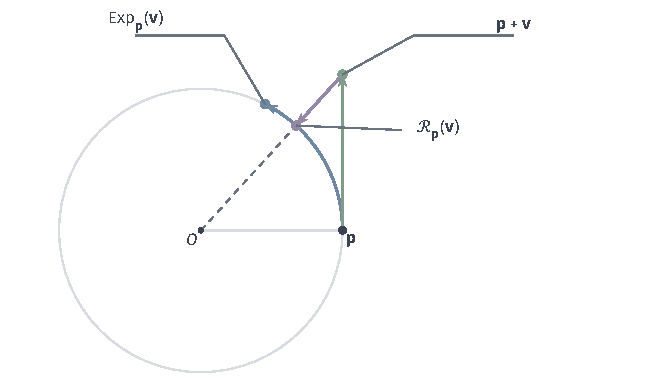
\includegraphics[width=112.0mm]{figures/00-shared/mathematical-preliminaries-upper/05-space-and-geometry/tikz/geometry-sphere-retraction/figure.pdf}
  \caption{单位圆截面中的切向步、指数映射与归一化回缩。
 取$\bm p=(1,0)^\top$、$\bm v=(0,1.1)^\top$。箭头为切向步，
 终点$\bm p+\bm v$位于圆外；紫色径向箭头将该点归一化为$\mathcal R_{\bm p}(\bm v)$。
 从起点方向计，蓝色指数更新转过$1.1$弧度，归一化回缩转过
 $\arctan(1.1)\approx0.833$弧度。两种更新关于步长的曲线在零步长处有相同初速度，
 但有限步位置不同。图为解析教学示例。}
 \label{fig:geometry-sphere-retraction}
\end{figure}
\FloatBarrier

\subsubsection{基于Newton与信赖域的二阶求解}
\label{sec:geometry-riemannian-newton-trust-region}

梯度只给局部下降方向，Hessian还能描述不同方向的二阶变化。
在当前点$\bm p$的切空间建立模型
\[
 m_{\bm p}(\bm\eta)=f(\bm p)
  +g(\operatorname{grad}f,\bm\eta)
  +\frac12g(\bm\eta,\operatorname{Hess}f[\bm\eta]).
\]
Newton方向解
$\operatorname{Hess}f[\bm\eta]=-\operatorname{grad}f$，
再用$\mathcal R_{\bm p}(\alpha\bm\eta)$更新。
取切空间正交归一基后，这是已有线性求解方法处理的对称系统；
一般坐标中可用式~\eqref{eq:geometry-hessian-coordinates}写成
$\bm B\bm\eta=-\nabla_{\bm z}f$。
Hessian奇异时方向可能不存在或不唯一，不定时Newton方向也可能不是下降方向。
局部快速收敛需要非退化解、足够光滑性、合适回缩和足够近的初始点，
不是二阶公式本身提供的全局保证。

信赖域方法限制模型适用范围，在$\lVert\bm\eta\rVert_g\leq\Delta$中近似最小化
$m_{\bm p}$。用实际下降与预测下降之比
\[
 \rho=\frac{f(\bm p)-f(\mathcal R_{\bm p}(\bm\eta))}
             {m_{\bm p}(\bm0)-m_{\bm p}(\bm\eta)}
\]
判断接受步和调整$\Delta$，只在分母为正时使用这个比值。
它允许利用负曲率方向，同时避免把远离当前点的模型误当成目标本身。
收敛结论仍需模型误差控制、子问题下降量及更新规则。

这里有一个二阶条件容易遗漏。令拉回目标
$\widehat f_{\bm p}(\bm\eta)=f(\mathcal R_{\bm p}(\bm\eta))$，
它定义在固定向量空间$T_{\bm p}\mathcal M$上。
回缩只保证其零点一阶导数等于$\mathrm df_{\bm p}$。
设$c(t)=\mathcal R_{\bm p}(t\bm\eta)$，由
式~\eqref{eq:geometry-function-second-derivative}，
\begin{equation}
 \frac{\mathrm d^2}{\mathrm dt^2}\widehat f_{\bm p}(t\bm\eta)
 \bigg|_{t=0}
 =g(\bm\eta,\operatorname{Hess}f[\bm\eta])
  +g(\operatorname{grad}f,D\dot c/\mathrm dt|_{t=0}).
 \label{eq:geometry-retraction-pullback-hessian}
\end{equation}
若回缩对所有$\bm\eta$均满足$D\dot c/\mathrm dt|_0=\bm0$，
称为二阶回缩（second-order retraction）。此时，或当前点已经驻定时，额外项才必定消失，
拉回目标的零点Hessian才与Riemann Hessian一致。
指数映射满足该条件；球面归一化回缩也满足，因为
$c''(0)=-\lVert\bm\eta\rVert_2^2\bm p$为纯法向。
对任意一阶回缩直接作二阶等同则不成立，
必须修正模型或另外证明所用模型满足算法的误差要求。
这些模型条件及一阶、二阶算法的收敛分析可参见Boumal的教材\scite{math-boumal2023optimization}。

若算法还复用前一步动量或搜索方向，它们位于旧切空间，不能与当前梯度直接相加。
可以沿已选路径作平行移动，也可指定较便宜的向量搬运（vector transport）
$\mathcal T_{\bm\eta}:T_{\bm p}\mathcal M\to
T_{\mathcal R_{\bm p}(\bm\eta)}\mathcal M$，
要求其对被搬运向量线性、随变量光滑且零步长时为恒等映射。
例如嵌入流形可投影旧方向到新切空间；这一般不保长度，甚至可能压掉某些方向，
并不是Levi--Civita平行移动。采用哪种搬运及它保留什么性质，
必须与具体迭代方法一起说明。

\section{收敛与逼近}
\label{sec:geometry-convergence-approximation}

这一节包含三类目标不同的收敛问题，不能用一个结论覆盖。
点序列回答极限是否仍属于流形；优化迭代还要受目标与更新规则支配；
有限采样回答样本能否恢复切平面、距离和拓扑。三者的误差尺度和条件互不相同，
最后一类依赖采样密度与噪声，这一差别是前面几节的直接延续。

\subsection{点序列的收敛}
\label{sec:geometry-point-convergence}

点序列$\bm p_n$收敛到$\bm p$，意味着$\bm p$的每个邻域最终包含全部$\bm p_n$。
在包含$\bm p$的坐标图中，这等价于坐标$\chi(\bm p_n)$趋于$\chi(\bm p)$：
坐标图及其逆连续，且序列最终留在该图内；嵌入模型中也等价于环境坐标收敛到流形内的$\bm p$。
极限必须属于原空间这一点不能省略：开单位圆弧上的点可以在环境中趋于被删去的端点，
却不在原空间中收敛。\BookSectionRef{sec:linear-algebra-sequence-convergence}{第\ref{sec:linear-algebra-sequence-convergence}节}说明有限维空间已由范数等价
保证了这些等价性，这里需要重新核对，是因为流形的坐标图只在局部有效。

Riemann距离给出相同的局部拓扑。取$\bm p$附近一个闭包仍在图内的小坐标球，
光滑正定度量的最小、最大特征值在其上分别有正下界和有限上界。
连接近点的坐标线段给出距离上界；任何离开这个小球的路径又必须付出正长度，
留在球内的路径长度则不小于坐标位移乘一个正系数。
所以足够近时坐标收敛与$d_g$收敛相互推出。
距离柯西列只保证点彼此越来越近；每个这样的列都有空间内极限才称完备。
定理~\ref{thm:geometry-hopf-rinow-existence}使用的正是这个条件，而不是坐标图覆盖的大小。

\subsection{点优化下的迭代序列收敛}
\label{sec:geometry-point-iteration-convergence}

回缩梯度法产生的序列还受目标与步长支配。设目标有下界$f_{\inf}$，且被接受的步满足
\[
 f(\bm p^{(k)})-f(\bm p^{(k+1)})\geq
 c\alpha^{(k)}\lVert\operatorname{grad}f(\bm p^{(k)})\rVert_g^2.
\]
求和后有
$\sum_k\alpha^{(k)}\lVert\operatorname{grad}f(\bm p^{(k)})\rVert_g^2
\leq(f(\bm p^{(0)})-f_{\inf})/c$。
若步长有统一正下界，就推出梯度范数趋零；
只知道步长趋零则不能作此推断。
在紧的下水平集上，若回缩光滑且拉回目标有统一的局部二阶界，
每步从同一个正试探步长开始、以固定比例回溯，就能让足够小的步长统一满足下降条件。
回溯会在这一统一尺度内停止，因此被接受的步长有正下界。
这些条件还确保更新留在回缩定义域内。

紧性保证有聚点；梯度连续使每个聚点驻定，却不自动保证所有迭代点趋于同一聚点，
也不把驻点变成全局最优。Newton局部快速收敛与信赖域全局驻点分析
还分别需要非退化性、模型一致性和子问题下降量条件。
因而收敛结论必须针对实际生成的序列陈述，不能由“在流形上使用梯度”单独推出。

\subsection{局部线性表示下的流形逼近}
\label{sec:geometry-local-linear-approximation}

切空间之所以适合近似，由Taylor展开说明。若参数化在当前邻域内二阶导数有界，则
\begin{equation}
 \varphi(\bm z+\bm h)-\varphi(\bm z)
 =\bm J_\varphi(\bm z)\bm h+O(\lVert\bm h\rVert_2^2).
 \label{eq:geometry-manifold-local-taylor}
\end{equation}
一阶项属于切空间，故环境位移投到法向正交补后只剩二阶余项。
这是局部结论，常数依赖所选邻域及二阶导数界；不能将它延伸到任意大步长。
法向偏离反映嵌入在环境中怎样弯曲，不等于第\ref{sec:geometry-riemannian-curvature}节定义的内在曲率。
在二维开带中法向空间为零，弯曲坐标线本身就不构成法向误差。


这里已知的是参数化曲面，用同一点的仿射切平面近似它。
二阶余项随坐标半径平方缩小；它是确定性局部偏差，不是样本协方差的统计误差。
仿射切平面本身可以无限延伸，近似保证却只在当前参数化与余项界有效的小邻域内成立。

\subsection{有限采样下的切空间逼近}
\label{sec:geometry-sampled-local-linearization}

只有$\bm x_i=\bm p_i+\bm\epsilon_i$时，参数化与潜在位置通常未知。
局部PCA（local principal component analysis）用邻域样本最主要的线性变化方向
估计真实切空间，是一种估计方法而不是流形的定义。
其直觉是：在一小块足够平的邻域内，点主要沿曲面自身的方向铺开，
垂直于曲面的方向只有小得多的弯曲偏离与噪声。把邻域内的散点当作一团数据，
沿哪些轴最分散，就对应沿曲面的切向；因此可以借用线性代数中“找最大方差方向”的PCA。
必须先说明潜在对象是二维带还是一维中心线，才能确定希望估计什么。

给观测$\bm x_i$选择邻居索引集$N_i$和权重
$\alpha_{i,j}\geq0$、$\sum_{j\in N_i}\alpha_{i,j}=1$，计算
\begin{equation}
 \overline{\bm x}_i=\sum_{j\in N_i}\alpha_{i,j}\bm x_j,\qquad
 \bm C_i=\sum_{j\in N_i}\alpha_{i,j}
  (\bm x_j-\overline{\bm x}_i)(\bm x_j-\overline{\bm x}_i)^\top.
 \label{eq:geometry-local-weighted-covariance}
\end{equation}
若潜在维数$d$给定，取$\bm C_i$最大$d$个特征值对应的正交特征向量
$\widehat{\bm U}_i$，其列空间$\widehat T_i$为估计方向子空间。
若$d$未知，需另由谱和误差模型判断；不能把预先指定的特征向量数当成维数发现。
局部均值消去样本位置偏移，但不保证等于$\bm p_i$。

这里有三个对象。$T_{\bm p_i}\mathcal M$是真实方向，
$\widehat T_i$是以零向量为原点的估计方向，
$\overline{\bm x}_i+\widehat T_i$或$\bm x_i+\widehat T_i$才是画出来的仿射近似。
若$d<D$，一般环境噪声使$\bm x_i\notin\mathcal M$，
此时$T_{\bm x_i}\mathcal M$甚至没有定义。
二维开带是当前例外：小噪声下观测仍在开带内，其切空间仍为$\mathbb R^2$，
但这不表示已经识别出生成它的潜在位置。

式~\eqref{eq:geometry-manifold-local-taylor}解释了误差来源。
在正则局部坐标中，邻域尺度为$h$时，切向位移通常为$O(h)$，
嵌入法向偏离为$O(h^2)$。若采样在各切方向上充分展开，
切向协方差特征值具有$h^2$量级；法向位移的平方贡献则可达到$h^4$量级。
这些尺度比较需要二阶导数有界和非退化局部采样，单靠光滑性并不保证谱间隙。


即使局部方向估计准确，也尚未得到全局坐标。圆的每个邻域只有一个切方向，
却不能以单张无断点实坐标图覆盖。局部PCA提供的是后续几何计算的局部输入，
不是全局展开或任务语义正确性的保证。

\subsection{有限采样下的距离逼近}
\label{sec:geometry-sampled-geodesic-distance}

只有观测点时，常把距离小于阈值$\varepsilon$的点相连，
或连接每个点的$k$个最近邻，再以$\lVert\bm x_i-\bm x_j\rVert_2$为边长。
一条边路径的长度是所经边长之和，最短边路径试图近似所选潜在流形上
$d_g(\bm p_i,\bm p_j)$。这里只借用顶点、边和路径的直观含义，
通用图算法留给\BookPartRef{part:discrete-mathematics-and-graph-theory}{第~\ref{part:discrete-mathematics-and-graph-theory}部分}。

潜在对象必须先定。若观测不在潜在流形上，$d_g(\bm x_i,\bm x_j)$便未定义；
即使观测在二维开带内，也不能因此把它认作$\bm p_i$。
环境欧氏边长自然对应欧氏诱导度量的局部近似；
若目标采用另一个Riemann度量，就要据此修正边长，不能继续沿用欧氏弦长而声称目标未变。

邻域要小到每条边只跨越近似平直的一段，避免从一折跳到另一折；
又要大到样本间的空隙能够连通。超过跨折环境间隔会引入捷径，低估沿潜在空间的距离；
小于采样空隙则会把一个真实分支拆开，返回无穷距离。
即使没有捷径，局部弦长误差与离散路径绕行误差也会共同作用，
不能无条件断言估计总在真实距离的同一侧。

固定$k$并不固定几何尺度。稀疏处第$k$个邻居可能很远，稠密处则很近，
有向近邻关系还可能不对称，需要声明如何对称化。
一致近似通常要求潜在流形光滑、采样在所研究区域逐渐稠密、
噪声相对邻域尺度受控，并让邻域半径随样本量缩小而仍足以覆盖采样空隙。
非紧开带若只在一部分采样，这些要求也只支持相应覆盖区域的结论。
具体收敛速度须结合采样分布与尺度选择证明，
最短边路径正确更不自动意味着后续全局坐标恢复正确。

\subsection{有限采样下的拓扑逼近}
\label{sec:geometry-sampled-topology-approximation}

固定同一组点和尺度，可以按共同覆盖或成对接近构造复形。
直觉上，用半径约为$\varepsilon/2$的小球盖住每个样本点：小球重叠，
说明这些点近到可以视为连续一片；重叠到什么程度，就决定该连边还是该填面。
把“球怎么重叠”翻译成纯组合规则，就得到下面两种复形；
它们只依赖点间距离，因而可以在没有已知曲面的情况下直接从样本构造。
\begin{definition}[Čech复形与Vietoris--Rips复形]
\label{def:geometry-cech-rips-complexes}
给定欧氏点集$\{\bm x_i\}$及$\varepsilon>0$，以
$B(\bm x_i,\varepsilon/2)$表示开球。
\term{Čech复形}（Čech complex）$\mathcal C_\varepsilon$纳入所有满足
$\bigcap_{i\in\sigma}B(\bm x_i,\varepsilon/2)\neq\varnothing$的非空顶点集$\sigma$。
\term{Vietoris--Rips复形}（Vietoris--Rips complex）$\mathcal R_\varepsilon$
纳入所有满足$\lVert\bm x_i-\bm x_j\rVert_2\leq\varepsilon$
对任意$i,j\in\sigma$成立的非空顶点集。
\end{definition}
这两种规则都向下封闭。Čech边要求距离严格小于$\varepsilon$，
Rips边在此采用不超过$\varepsilon$的约定；开闭边界的差异须在临界尺度明确保留。
更本质的差别出现在三点以上：成对相交不保证共同交集。

例如$\varepsilon=1$、边长$0.9$的正三角形，三对半径$0.5$的球均相交，
因此Rips加入三角面。覆盖三个顶点的最小球半径却是$0.9/\sqrt3>0.5$，
不存在三个球的共同交点，Čech只保留三条边。
图~\ref{fig:geometry-cech-rips-intersection}中的中心叉号给出这个最小覆盖半径，
不是利用开闭球的等号差异制造反例。
\begin{figure}[htbp]
  \centering
  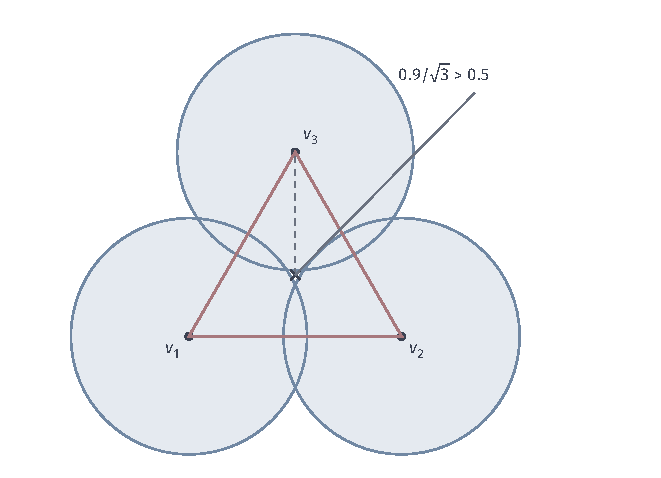
\includegraphics[width=112.0mm]{figures/00-shared/mathematical-preliminaries-upper/05-space-and-geometry/tikz/geometry-cech-rips-intersection/figure.pdf}
  \caption{固定同组三点比较共同交集与成对条件。正三角形边长$0.9$，
 $\varepsilon=1$，蓝色开球半径$0.5$；红色边满足两种构造的连边条件。
 三球无共同交点，Čech不含二维面，Rips含二维面。
 中心到各顶点的距离为$0.9/\sqrt3>0.5$。圆周只标开球边界，图为解析教学构造。}
 \label{fig:geometry-cech-rips-intersection}
\end{figure}

尺度变化后仍可给出明确包含关系。对任意$\eta>0$，有
\[
 \mathcal C_\varepsilon\subseteq\mathcal R_\varepsilon
 \subseteq\mathcal C_{2\varepsilon+\eta}.
\]
第一个包含关系由共同交点和三角不等式推出。
对第二个，任选一个顶点作候选共同交点，它到其余顶点的距离至多$\varepsilon$，
严格小于新球半径$\varepsilon+\eta/2$。
若全部球改用闭球，在相应定义下可取尺度常数$2$而不加$\eta$。
这些是足够的普适常数，不声称最紧；同一尺度的复形仍不能互换。

复形何时能代表球并集的拓扑，还依赖覆盖条件。良好覆盖（good cover）要求每个
非空有限交集都可连续收缩到一点；有限欧氏开球的交集为凸集，满足这项要求。
神经引理（nerve lemma）在该条件下说明Čech复形的几何实现$|\mathcal C_\varepsilon|$
与球并集同伦等价，即二者存在相互连续映射，
来回复合可以连续变形到恒等映射。这里不要求两映射互为逆，所以比同胚弱：
闭区间可连续收缩到一个点，与单点空间同伦等价，却不可能与它存在双射。
这个结论不等于球并集已经恢复了未知潜在流形；
后者还需要采样覆盖和尺度条件。


复形的规模还依赖邻域尺度。开带$\mathcal M_{\mathrm{strip}}$与开矩形同胚，
中心线$\mathcal C$与开区间同胚，都没有全局环。
闭合中心线得到圆，保留横向自由度并闭合则得到二维环带；
维数不同，但都保留绕中心的一维环。只有在采样和尺度适当时，样本复形才有理由
反映这些区别。尺度太小会把采样空隙误认作分支；太大则可能跨折连边，
并以高阶面填掉原来的环。

持续同调（persistent homology）跟踪随尺度增大而嵌套的复形中，同调类何时出现、
何时消失；它提供跨尺度信息，不使所有长寿命结构自动具有真实任务语义。
之所以要看“随尺度变化”，是因为单一尺度的答案常常不稳定：尺度稍小，
真环可能被样本缺口截断；尺度稍大，捷径又可能把洞填上。
让尺度从$0$连续增大，观察一个环在多大尺度上诞生、又在多大尺度上被填充，
存活跨度因而比某一张快照提供更多跨尺度证据。但长寿命环也可能来自系统性的采样偏差，
不能仅凭寿命就判定它是真实孔洞；把这些结构解释为潜在对象的拓扑，仍需核验采样覆盖、
噪声大小与所选尺度，并使用相应的稳定性或恢复条件。


固定阈值时，若一对点的距离由阈值以下扰动到阈值以上，相应的边会突然消失。软关系改用
$\mu_{i,j}\in[0,1]$表示所选局部尺度下的邻接支持强度；
这只是隶属度，不自动是事件概率。若两个点各按自己的局部尺度确定邻居，
同一对点可能得到不同的有向强度。令$a=\mu_{i,j}$、$b=\mu_{j,i}$，
可以把二者合成一条无向边的强度。一种合并规则是
\begin{equation}
 a\mathbin{\sqcup}b=a+b-ab=1-(1-a)(1-b),\qquad a,b\in[0,1].
 \label{eq:geometry-fuzzy-union}
\end{equation}
例如$a=0.6$、$b=0.5$时，无向强度为$0.8$，表示按此规则综合两端的邻接支持。
高阶面的强度还需另定规则，例如取其全部边强度的最小值，并不由这个二元运算自动给出。
合并结果仍在$[0,1]$内；交换性由对称式给出，结合性由
$1-(1-a)(1-b)(1-c)$给出，$0$为恒等元，任一输入为$1$时输出为$1$。
这些性质使它成为明确定义的软并集，却没有提供独立事件的随机试验或联合分布。
核权重、相似度、置信度与概率的校准要求不能仅凭数值范围混同。

UMAP等方法由局部距离构造带强度的关系，再优化低维坐标以匹配这些关系；
具体目标与优化过程可参考
\BookChapterRef{chap:dimensionality-reduction}{卷4《模型：经典模型》第5章“降维”}。
低维图像中的分离簇或孔洞还可能受邻居数、尺度、初始化与优化误差影响。
拓扑方法不能修复错误的局部输入：跨折捷径会被忠实组合，完全漏采的区域也无法凭空
恢复。采样覆盖、局部关系与尺度共同限制结论。

\section{扰动与稳定性}
\label{sec:geometry-stability}

上一节讨论的是缩小邻域、增加采样怎样改善逼近；这里问的是另一件事：
观测或计算稍变以后，输出会变多少。两者不能互相替代，逼近误差不随之消失。
本章要比较的输出有四种，各自的尺度不同：映射输出用坐标距离，
切空间估计用子空间夹角，重构坐标用点云距离，路径解用固定时间上的状态差。
前三者还要先消去记录本身的任意性（换基、整体旋转平移、点标签），
否则量到的是记录差异而非问题响应。

\subsection{运算的误差传播}
\label{sec:geometry-operation-stability}

对光滑点映射$F$，记其局部坐标表达为$\widehat F$。
在一个凸坐标区域上设$\lVert\bm J_{\widehat F}\rVert_2\leq L$，
沿区域内的线段积分得到
$\lVert\widehat F(\bm z+\bm h)-\widehat F(\bm z)\rVert_2
\leq L\lVert\bm h\rVert_2$。
跨图时还需计入两端坐标转换及度量的上下界；一个坐标中的小扰动不是坐标无关的数值。
叠加的局部放大界不超过$\sum_j|a_j|L_j$，复合不超过各步界的乘积。
若归一化分母趋零、参数化Jacobian接近降秩，这些界会变差，
因此合法运算与数值稳定是两个需要分别核对的条件。

\subsection{切空间估计的稳定性}
\label{sec:geometry-tangent-estimate-stability}

局部PCA从协方差矩阵选出一个子空间。为比较它与真实切空间，
先以潜在点处的一阶切向位移构造理想协方差$\bm C_0$，
并假设采样在全部$d$个切方向上都有变化；这样$\bm C_0$的前$d$维特征子空间才是真实切空间。
设实际协方差为$\bm C_0+\bm E$，用正交投影$\bm P$、$\widehat{\bm P}$
分别表示真实与估计子空间。两投影之差的算子范数衡量最大方向偏差，
等于\BookDefinitionRef{def:matrix-analysis-principal-angles}{定义~\ref{def:matrix-analysis-principal-angles}}中最大主角的正弦，且不受各自基选择影响。

当$d<D$时，把$\bm C_0$的特征值降序排列，设
$\delta=\lambda_d-\lambda_{d+1}>0$，并要求$\lVert\bm E\rVert_2<\delta/2$。
\BookSectionRef{sec:linear-algebra-spectral-stability}{第~\ref{sec:linear-algebra-spectral-stability}节}的单侧谱隙界和Weyl界给出
\[
 \lVert\widehat{\bm P}-\bm P\rVert_2
 \leq\frac{\lVert\bm E\rVert_2}{\delta-\lVert\bm E\rVert_2}
 \leq\frac{2\lVert\bm E\rVert_2}{\delta}.
\]
这里$\bm E$包括有限样本波动、噪声、邻域错选及非线性近似误差，
不能只代入测量噪声方差；若理想协方差未在全部切方向上展开，也不能把它的主子空间认作真实切空间。
若已知$d=D$，目标切空间就是整个环境空间$\mathbb R^D$，
无需用这条谱隙辨认方向；维数是否确为$D$仍是另一个模型判断。

缩小邻域会降低法向二阶偏差，却减少样本并压低真实信号的谱尺度；
固定噪声不会随之自动消失。邻域过大时，中心线不同位置的切线已明显转动，
PCA得到的是折中方向。对二维窄带，若样本的横向覆盖不足或宽度小于噪声尺度，
第二个方向可能难以稳定识别，但潜在对象并不因此变成一维。
固定近邻数也不能解决非均匀密度带来的变化：稀疏处覆盖范围大，稠密处范围小。
潜在对象、采样密度、嵌入弯曲、邻域尺度、谱间隙和噪声必须一起解释。


估计子空间内部的基可以旋转，输出应比较投影或主角，而不是逐列比较特征向量。
谱隙、邻域尺度和噪声一起决定能否区分切向与法向；增加样本数量不能消除固定尺度带来的几何偏差。

\subsection{坐标重构的稳定性}
\label{sec:geometry-coordinate-reconstruction-stability}

设平方距离矩阵由$\bm\Delta$变成$\bm\Delta+\bm E$。
中心化矩阵$\bm J$是正交投影，故重构Gram矩阵的扰动为
\[
 \widetilde{\bm B}-\bm B=-\tfrac12\bm J\bm E\bm J,\qquad
 \lVert\widetilde{\bm B}-\bm B\rVert_2\leq\tfrac12\lVert\bm E\rVert_2.
\]
\BookSectionRef{sec:linear-algebra-spectral-stability}{第\ref{sec:linear-algebra-spectral-stability}节}的谱扰动结论控制特征值与选定谱子空间。
选取前$d$维坐标时，需要$d$与$d+1$模态之间的谱隙；
对正特征值开平方还需要它们远离零。接近零的模态可能改变保留维数，
重复特征值则允许同一子空间内任意转动。

比较坐标前应先消去平移，再允许整体正交对齐，因为距离本来就不识别这些变换。
若点标签也改变，还须先建立点对应。小距离扰动只能在上述尺度与对齐条件下
支持坐标稳定，不能保证某个优化过程恰好返回同一朝向的坐标。

\subsection{拓扑重构的稳定性}
\label{sec:geometry-topology-reconstruction-stability}

固定阈值构造的单个复形可能发生跳变。若成对距离误差不超过$\delta$，
所有距离原本小于$\varepsilon-\delta$的边仍会被纳入，
原本大于$\varepsilon+\delta$的边仍会被排除；处在中间带内的边不能保证。
对Rips复形，这直接给出
$\mathcal R_{\varepsilon-\delta}\subseteq\widetilde{\mathcal R}_{\varepsilon}
\subseteq\mathcal R_{\varepsilon+\delta}$（左侧只在正尺度使用）。
固定尺度上的Betti数仍可能变化；跨尺度比较能把不确定性记录为尺度偏移，
但具体持续图距离的界还需要所用过滤的稳定性定理。
完全漏采的区域、错误点对应或大幅跨折连边并不属于小扰动假设，
不能从局部稳定性恢复其中的信息。

\subsection{路径解的稳定性}
\label{sec:geometry-path-solution-stability}

初值问题同时更新位置与速度。把状态记为$\bm y=(\bm z,\dot{\bm z})$以后，
它在一张坐标图中成为一阶系统$\bm y'=A(\bm y)$；
$A$由测地线方程中的速度与加速度组成。
设另一方程为$\widetilde{\bm y}'=\widetilde A(\widetilde{\bm y})$。
若两条解留在同一紧区域$K$，$A$在该区域有Lipschitz常数$L$，
且$\sup_{\bm y\in K}\lVert A(\bm y)-\widetilde A(\bm y)\rVert\leq\eta$，
积分方程给出
\[
 \lVert \bm y(t)-\widetilde{\bm y}(t)\rVert
 \leq e^{Lt}\lVert \bm y(0)-\widetilde{\bm y}(0)\rVert
       +\eta\int_0^t e^{L(t-s)}\,\mathrm ds,\qquad t\geq0.
\]
这是Gronwall不等式的直接应用，比较的是固定时间区间上的初值轨迹。
一旦路径离开该区域，常数与比较图都须重新核对。

固定端点的最短路有不同边界：距离作为最小代价可能连续，
达到它的路线却未必唯一。球面上到对跖点的最短路有多条；
终点向不同方向稍微偏离，会选出不同的大圆弧。
若局部有唯一最短路且避开使端点映射退化的位置，才可利用指数映射的局部逆
控制路线对端点的响应。初值唯一性不能替代端点最短路的稳定性条件。

\section{本章小结}
\label{sec:geometry-summary}

本章把非线性对象的局部记录、关系、运算、求解、逼近与稳定性分开建立。
坐标图记录位置，切空间规定瞬时方向，度量读出长度，路径长度的下确界定义距离；
等价关系则明确哪些输入变化被主动忽略。局部自由度、环境维数和有限观测不是同一对象。
比例等价给出射影空间，仿射图把其中一部分变成普通坐标；无穷远只是相对于该图的未覆盖方向。
点线关联可由齐次方程保留，点对应估计则还要检查一般位置、尺度选择及矩阵可逆性。

映射微分传递速度，联络与平行移动比较不同位置的方向，指数映射和回缩产生可行的新点。
给定初值求轨迹与给定端点求最短路有不同的唯一性、存在性和稳定性边界。
点优化调用这些运算选择更新，其下降、驻点与点序列收敛仍须分别证明。
SO(3)把切向限制为斜对称生成元，Rodrigues公式计算合法旋转；
四元数的单位约束和双覆盖又说明连续记录并不等于全局唯一坐标。
最短弧插值须选择代表符号，并在半周旋转处保留路径歧义；
SE(3)的平移还随旋转复合，不能脱离坐标方向直接相加。

局部切平面、样本PCA、最短边路径和复形各自逼近方向、距离或拓扑。
尺度、覆盖、谱隙与噪声决定适用范围；环境弯曲、内在曲率和整体孔洞不能互相替代。
下一章把整个函数作为可变对象，沿用这里的几何域、微分与体积，
研究函数读取、函数拟合以及平滑能量所决定的函数与场优化。

